%%%%%%%%%%%%%%%%%%%%%%%%%%%%%%%%%%%%%%%%
% datoteka diploma-FRI-vzorec.tex
%
% vzorčna datoteka za pisanje diplomskega dela v formatu LaTeX
% na UL Fakulteti za računalništvo in informatiko
%
% na osnovi starejših verzij vkup spravil Franc Solina, maj 2021
% prvo verzijo je leta 2010 pripravil Gašper Fijavž
%
% za upravljanje z literaturo ta vezija uporablja BibLaTeX
%
% svetujemo uporabo Overleaf.com - na tej spletni implementaciji LaTeXa ta vzorec zagotovo pravilno deluje
%

\documentclass[a4paper,12pt,openright]{book}
%\usepackage{listings}
%\usepackage{xcolor}
%\lstset { %
%    language=C++,
%    backgroundcolor=\color{black!5}, % set backgroundcolor
%    basicstyle=\footnotesize,% basic font setting
%}
%\documentclass[a4paper, 12pt, openright, draft]{book}  Nalogo preverite tudi z opcijo draft, ki pokaže, katere vrstice so predolge! Pozor, v draft opciji, se slike ne pokažejo!
 
\usepackage[utf8]{inputenc}   % omogoča uporabo slovenskih črk kodiranih v formatu UTF-8
\usepackage[slovene,english]{babel}    % naloži, med drugim, slovenske delilne vzorce
\usepackage[pdftex]{graphicx}  % omogoča vlaganje slik različnih formatov
\usepackage{fancyhdr}          % poskrbi, na primer, za glave strani
\usepackage{amssymb}           % dodatni matematični simboli
\usepackage{amsmath}           % eqref, npr.
\usepackage{hyperxmp}
\usepackage[hyphens]{url}
\usepackage{csquotes}
\usepackage[pdftex, colorlinks=true,
						citecolor=black, filecolor=black, 
						linkcolor=black, urlcolor=black,
						pdfproducer={LaTeX}, pdfcreator={LaTeX}]{hyperref}

\usepackage{color}
\usepackage{soul}
\usepackage[dvipsnames]{xcolor}
\usepackage{dirtree}
\usepackage{minted}
\usepackage{tikz}
\usepackage{siunitx}
\usetikzlibrary{shapes, positioning, matrix}
\usepackage[
backend=biber,
style=numeric,
sorting=nty,
]{biblatex}


\addbibresource{literatura.bib} %Imports bibliography file


%%%%%%%%%%%%%%%%%%%%%%%%%%%%%%%%%%%%%%%%
%	DIPLOMA INFO
%%%%%%%%%%%%%%%%%%%%%%%%%%%%%%%%%%%%%%%%
\newcommand{\ttitle}{Razvoj vgrajenega podatkovnega sistema}
\newcommand{\ttitleEn}{Diploma thesis template}
\newcommand{\tsubject}{\ttitle}
\newcommand{\tsubjectEn}{\ttitleEn}
\newcommand{\tauthor}{Janez Sedeljšak}
\newcommand{\tkeywords}{Podatkovne baze, C++, Python, B+ drevesa, Podatkovne strukture}
\newcommand{\tkeywordsEn}{Databases, C++, Python, B+ trees, Data structures}

%%%%%%%%%%%%%%%%%%%%%%%%%%%%%%%%%%%%%%%%
%	HYPERREF SETUP
%%%%%%%%%%%%%%%%%%%%%%%%%%%%%%%%%%%%%%%%
\hypersetup{pdftitle={\ttitle}}
\hypersetup{pdfsubject=\ttitleEn}
\hypersetup{pdfauthor={\tauthor}}
\hypersetup{pdfkeywords=\tkeywordsEn}

%%%%%%%%%%%%%%%%%%%%%%%%%%%%%%%%%%%%%%%%
% postavitev strani
%%%%%%%%%%%%%%%%%%%%%%%%%%%%%%%%%%%%%%%%  

\addtolength{\marginparwidth}{-20pt} % robovi za tisk
\addtolength{\oddsidemargin}{40pt}
\addtolength{\evensidemargin}{-40pt}

\renewcommand{\baselinestretch}{1.3} % ustrezen razmik med vrsticami
\setlength{\headheight}{15pt}        % potreben prostor na vrhu
\renewcommand{\chaptermark}[1]%
{\markboth{\MakeUppercase{\thechapter.\ #1}}{}} \renewcommand{\sectionmark}[1]%
{\markright{\MakeUppercase{\thesection.\ #1}}} \renewcommand{\headrulewidth}{0.5pt} \renewcommand{\footrulewidth}{0pt}
\fancyhf{}
\fancyhead[LE,RO]{\sl \thepage} 
%\fancyhead[LO]{\sl \rightmark} \fancyhead[RE]{\sl \leftmark}
\fancyhead[RE]{\sc \tauthor}              % dodal Solina
\fancyhead[LO]{\sc Diplomska naloga}     % dodal Solina


\newcommand{\BibLaTeX}{{\sc Bib}\LaTeX}
\newcommand{\BibTeX}{{\sc Bib}\TeX}

%%%%%%%%%%%%%%%%%%%%%%%%%%%%%%%%%%%%%%%%
% naslovi
%%%%%%%%%%%%%%%%%%%%%%%%%%%%%%%%%%%%%%%%  

\newcommand{\autfont}{\Large}
\newcommand{\titfont}{\LARGE\bf}
\newcommand{\clearemptydoublepage}{\newpage{\pagestyle{empty}\cleardoublepage}}
\setcounter{tocdepth}{1}	      % globina kazala

%%%%%%%%%%%%%%%%%%%%%%%%%%%%%%%%%%%%%%%%
% konstrukti
%%%%%%%%%%%%%%%%%%%%%%%%%%%%%%%%%%%%%%%%  
\newtheorem{izrek}{Izrek}[chapter]
\newtheorem{trditev}{Trditev}[izrek]
\newenvironment{dokaz}{\emph{Dokaz.}\ }{\hspace{\fill}{$\Box$}}


%%%%%%%%%%%%%%%%%%%%%%%%%%%%%%%%%%%%%%%%%%%%%%%%%%%%%%%%%%%%%%%%%%%%%%%%%%%%%%%
%% PDF-A
%%%%%%%%%%%%%%%%%%%%%%%%%%%%%%%%%%%%%%%%%%%%%%%%%%%%%%%%%%%%%%%%%%%%%%%%%%%%%%%

%%%%%%%%%%%%%%%%%%%%%%%%%%%%%%%%%%%%%%%% 
% define medatata
%%%%%%%%%%%%%%%%%%%%%%%%%%%%%%%%%%%%%%%% 
\def\Title{\ttitle}
\def\Author{\tauthor, js0578@student.uni-lj.si}
\def\Subject{\ttitleEn}
\def\Keywords{\tkeywordsEn}

%%%%%%%%%%%%%%%%%%%%%%%%%%%%%%%%%%%%%%%% 
% \convertDate converts D:20080419103507+02'00' to 2008-04-19T10:35:07+02:00
%%%%%%%%%%%%%%%%%%%%%%%%%%%%%%%%%%%%%%%% 
\def\convertDate{%
    \getYear
}

{\catcode`\D=12
 \gdef\getYear D:#1#2#3#4{\edef\xYear{#1#2#3#4}\getMonth}
}
\def\getMonth#1#2{\edef\xMonth{#1#2}\getDay}
\def\getDay#1#2{\edef\xDay{#1#2}\getHour}
\def\getHour#1#2{\edef\xHour{#1#2}\getMin}
\def\getMin#1#2{\edef\xMin{#1#2}\getSec}
\def\getSec#1#2{\edef\xSec{#1#2}\getTZh}
\def\getTZh +#1#2{\edef\xTZh{#1#2}\getTZm}
\def\getTZm '#1#2'{%
    \edef\xTZm{#1#2}%
    \edef\convDate{\xYear-\xMonth-\xDay T\xHour:\xMin:\xSec+\xTZh:\xTZm}%
}

%\expandafter\convertDate\pdfcreationdate 

%%%%%%%%%%%%%%%%%%%%%%%%%%%%%%%%%%%%%%%%
% get pdftex version string
%%%%%%%%%%%%%%%%%%%%%%%%%%%%%%%%%%%%%%%% 
\newcount\countA
\countA=\pdftexversion
\advance \countA by -100
\def\pdftexVersionStr{pdfTeX-1.\the\countA.\pdftexrevision}


%%%%%%%%%%%%%%%%%%%%%%%%%%%%%%%%%%%%%%%%
% XMP data
%%%%%%%%%%%%%%%%%%%%%%%%%%%%%%%%%%%%%%%%  
\usepackage{xmpincl}
%\includexmp{pdfa-1b}

%%%%%%%%%%%%%%%%%%%%%%%%%%%%%%%%%%%%%%%%
% pdfInfo
%%%%%%%%%%%%%%%%%%%%%%%%%%%%%%%%%%%%%%%%  
\pdfinfo{%
    /Title    (\ttitle)
    /Author   (\tauthor, js0578@student.uni-lj.si)
    /Subject  (\ttitleEn)
    /Keywords (\tkeywordsEn)
    /ModDate  (\pdfcreationdate)
    /Trapped  /False
}

%%%%%%%%%%%%%%%%%%%%%%%%%%%%%%%%%%%%%%%%
% znaki za copyright stran
%%%%%%%%%%%%%%%%%%%%%%%%%%%%%%%%%%%%%%%%  

\newcommand{\CcImageCc}[1]{%
	\includegraphics[scale=#1]{cc_cc_30.pdf}%
}
\newcommand{\CcImageBy}[1]{%
	\includegraphics[scale=#1]{cc_by_30.pdf}%
}
\newcommand{\CcImageSa}[1]{%
	\includegraphics[scale=#1]{cc_sa_30.pdf}%
}

%%%%%%%%%%%%%%%%%%%%%%%%%%%%%%%%%%%%%%%%%%%%%%%%%%%%%%%%%%%%%%%%%%%%%%%%%%%%%%%
%%%%%%%%%%%%%%%%%%%%%%%%%%%%%%%%%%%%%%%%%%%%%%%%%%%%%%%%%%%%%%%%%%%%%%%%%%%%%%%

\begin{document}
\selectlanguage{slovene}
\frontmatter
\setcounter{page}{1} %
\renewcommand{\thepage}{}       % preprečimo težave s številkami strani v kazalu

%%%%%%%%%%%%%%%%%%%%%%%%%%%%%%%%%%%%%%%%
%naslovnica
 \thispagestyle{empty}%
   \begin{center}
    {\large\sc Univerza v Ljubljani\\%
%      Fakulteta za elektrotehniko\\% za študijski program Multimedija
%      Fakulteta za upravo\\% za študijski program Upravna informatika
      Fakulteta za računalništvo in informatiko\\%
%      Fakulteta za matematiko in fiziko\\% za študijski program Računalništvo in matematika
     }
    \vskip 10em%
    {\autfont \tauthor\par}%
    {\titfont \ttitle \par}%
    {\vskip 3em \textsc{DIPLOMSKO DELO\\[5mm]         % dodal Solina za ostale študijske programe
    VISOKOŠOLSKI STROKOVNI ŠTUDIJSKI PROGRAM\\ PRVE STOPNJE\\ RAČUNALNIŠTVO IN INFORMATIKA}\par}%
%     UNIVERZITETNI  ŠTUDIJSKI PROGRAM\\ PRVE STOPNJE\\ RAČUNALNIŠTVO IN INFORMATIKA}\par}%
%    INTERDISCIPLINARNI UNIVERZITETNI\\ ŠTUDIJSKI PROGRAM PRVE STOPNJE\\ MULTIMEDIJA}\par}%
%    INTERDISCIPLINARNI UNIVERZITETNI\\ ŠTUDIJSKI PROGRAM PRVE STOPNJE\\ UPRAVNA INFORMATIKA}\par}%
%    INTERDISCIPLINARNI UNIVERZITETNI\\ ŠTUDIJSKI PROGRAM PRVE STOPNJE\\ RAČUNALNIŠTVO IN MATEMATIKA}\par}%
    \vfill\null%
% izberite pravi habilitacijski naziv mentorja!
    {\large \textsc{Mentor}: doc. dr. Boštjan Slivnik\par}%
    {\vskip 2em \large Ljubljana, \the\year \par}%
\end{center}
% prazna stran
%\clearemptydoublepage      
% izjava o licencah itd. se izpiše na hrbtni strani naslovnice

%%%%%%%%%%%%%%%%%%%%%%%%%%%%%%%%%%%%%%%%
%copyright stran
%%%%%%%%%%%%%%%%%%%%%%%%%%%%%%%%%%%%%%%%
\newpage
\thispagestyle{empty}

\vspace*{5cm}
{\small \noindent
To delo je ponujeno pod licenco \textit{Creative Commons Priznanje avtorstva-Deljenje pod enakimi pogoji 2.5 Slovenija} (ali novej\v so razli\v cico).
To pomeni, da se tako besedilo, slike, grafi in druge sestavine dela kot tudi rezultati diplomskega dela lahko prosto distribuirajo,
reproducirajo, uporabljajo, priobčujejo javnosti in predelujejo, pod pogojem, da se jasno in vidno navede avtorja in naslov tega
dela in da se v primeru spremembe, preoblikovanja ali uporabe tega dela v svojem delu, lahko distribuira predelava le pod
licenco, ki je enaka tej.
Podrobnosti licence so dostopne na spletni strani \href{http://creativecommons.si}{creativecommons.si} ali na Inštitutu za
intelektualno lastnino, Streliška 1, 1000 Ljubljana.

\vspace*{1cm}
\begin{center}% 0.66 / 0.89 = 0.741573033707865
%{ \CcImageCc{0.741573033707865}\hspace*{1ex}\CcImageBy{1}\hspace*{1ex}\CcImageSa{1}% }%
\end{center}
}

\vspace*{1cm}
{\small \noindent
Izvorna koda diplomskega dela, njeni rezultati in v ta namen razvita programska oprema je ponujena pod licenco GNU General Public License,
različica 3 (ali novejša). To pomeni, da se lahko prosto distribuira in/ali predeluje pod njenimi pogoji.
Podrobnosti licence so dostopne na spletni strani \url{http://www.gnu.org/licenses/}.
}

\vfill
\begin{center} 
\ \\ \vfill
{\em
Besedilo je oblikovano z urejevalnikom besedil \LaTeX.}
\end{center}

% prazna stran
\clearemptydoublepage

%%%%%%%%%%%%%%%%%%%%%%%%%%%%%%%%%%%%%%%%
% stran 3 med uvodnimi listi
\thispagestyle{empty}
\
\vfill

\bigskip
\noindent\textbf{Kandidat:} Janez Sedeljšak\\
\noindent\textbf{Naslov:} Razvoj vgrajenega podatkovnega sistema\\
\noindent\textbf{Vrsta naloge:} Diplomska naloga na visokošolskem programu prve stopnje Računalništvo in informatika \\
\noindent\textbf{Mentor:} doc. dr. Boštjan Slivnik\\

\bigskip
\noindent\textbf{Opis:}\\
Besedilo teme diplomskega dela študent prepiše iz študijskega informacijskega sistema, kamor ga je vnesel mentor. 
V nekaj stavkih bo opisal, kaj pričakuje od kandidatovega diplomskega dela. 
Kaj so cilji, kakšne metode naj uporabi, morda bo zapisal tudi ključno literaturo.

\bigskip
\noindent\textbf{Title:} Development of an embeded database system

\bigskip
\noindent\textbf{Description:}\\
opis diplome v angleščini

\vfill



\vspace{2cm}

% prazna stran
\clearemptydoublepage

% zahvala
%\thispagestyle{empty}\mbox{}\vfill\null\it%
%\noindent
%Na tem mestu zapišite, komu se zahvaljujete za pomoč pri izdelavi diplomske naloge oziroma pri vašem študiju %nasploh. Pazite, da ne boste koga pozabili. Utegnil vam bo zameriti. Temu se da izogniti tako, da celotno %zahvalo izpustite.
%$\rm\normalfont

% prazna stran
\clearemptydoublepage

%%%%%%%%%%%%%%%%%%%%%%%%%%%%%%%%%%%%%%%%
% posvetilo, če sama zahvala ne zadošča :-)
%\thispagestyle{empty}\mbox{}{\vskip0.20\textheight}\mbox{}\hfill\begin{minipage}{0.55\textwidth}%
%Svoji dragi Alenčici.
%\normalfont\end{minipage}

% prazna stran
\clearemptydoublepage


%%%%%%%%%%%%%%%%%%%%%%%%%%%%%%%%%%%%%%%%
% kazalo
\setcounter{tocdepth}{4}
\pagestyle{empty}
\def\thepage{}% preprečimo težave s številkami strani v kazalu
\tableofcontents{}


% prazna stran
\clearemptydoublepage

%%%%%%%%%%%%%%%%%%%%%%%%%%%%%%%%%%%%%%%%
% seznam kratic

\chapter*{Seznam uporabljenih kratic}

\noindent\begin{tabular}{p{0.2\textwidth}|p{.35\textwidth}|p{.35\textwidth}}    % po potrebi razširi prvo kolono tabele na račun drugih dveh!
  {\bf kratica} & {\bf angleško}                              & {\bf slovensko} \\ \hline
  {\bf DBMS} & database management system & sistem za upravljanje podatkovnih baz \\
  {\bf API} & application programming interface & aplikacijski programski vmesnik \\
  {\bf SQL} & structured query language & strukturiran jezik poizvedb \\
  {\bf NoSQL} & nerelacijske podatkovne baze & nonrelational databases \\
  {\bf I/O} & input/output operations & vhodno/izhodne operacije \\
  {\bf SSD} & solid-state drive & negiljivi diski \\
  {\bf ER} & entitiy relationship (diagram) & (diagram) entitet in relaciji \\
  {\bf ORM} & object-relational mapping & objektno relacijska preslikava \\
  {\bf HTTP} & hypertext transfer protocol & protokol za prenos hiperteksta \\
  {\bf CLI} & command line interface & vmesnik za ukazno vrstico \\
  {\bf CI/CD} & continuous integration, continuous delivery & neprekinjena integracija in postavitev \\
  {\bf CSV} & comma-separated values & vrednosti, ločene z vejico \\
%  \dots & \dots & \dots \\
\end{tabular}


% prazna stran
\clearemptydoublepage

%%%%%%%%%%%%%%%%%%%%%%%%%%%%%%%%%%%%%%%%
% povzetek
\phantomsection
\addcontentsline{toc}{chapter}{Povzetek}
\chapter*{Povzetek}

\noindent\textbf{Naslov:} \ttitle
\bigskip

\noindent\textbf{Avtor:} \tauthor
\bigskip

%\noindent\textbf{Povzetek:} 
\noindent V diplomskem delu je predstavljenih trenutno nekaj najbolj uporabljenih relacijskih podatkovnih sistemov (DMBS). V veliki meri so standard podatkovnih baz še vedno relacijske podatkovne baze. V ta namen je tekom dela predstavljen razvoj vgrajenega relacijskega sistema za programski jezik Python.

Sam razvoj namenske knjižnice je pripravljen v programskem jeziku C++, saj gre za nizko nivojski jezik, kjer imamo visoko fleksibilnost pri upravljanju s pomnilniku. Predstavljen je razvoj vseh potrebnih segmentov za dobro delujočo relacijsko podatkovno bazo. Ključnega pomena tekom razvoja je bila uporaba dobrih podatkovnih struktur in algoritmov, ki dobro izkoristijo I/O operacije, ki jih ponuja operacijski sistem in posledično pripeljejo do dobro pripravljenega podatkovnega sistema.

V zadnjem sklopu diplomskega dela smo pripravili analizo uspešnosti implementacije podatkovnega sistema na različnih scenarijih in ob različnih konfiguracijah. Poleg tega je pripravljena tudi analiza z že obstoječimi DMBS – SQLite in MySQL) ob enakovrednih scenarijih testiranja novo pripravljene knjižnice.
\bigskip

\noindent\textbf{Ključne besede:} \tkeywords.
% prazna stran
\clearemptydoublepage

%%%%%%%%%%%%%%%%%%%%%%%%%%%%%%%%%%%%%%%%
% abstract
\phantomsection
\selectlanguage{english}
\addcontentsline{toc}{chapter}{Abstract}
\chapter*{Abstract}

\noindent\textbf{Title:} \ttitleEn
\bigskip

\noindent\textbf{Author:} \tauthor
\bigskip

%\noindent\textbf{Abstract:} 
\noindent The thesis presents several currently used relational systems for working with data (DBMS). Relational databases are still widely used as the standard data storage systems. In this context, the development of an embedded relational database system for the Python programming language is presented.

The development of the dedicated library is implemented in the C++ programming language, which is a low-level language providing high flexibility in memory management. The development of all necessary components for a well-functioning relational database is described. During the development process, a key focus was on utilizing efficient data structures and algorithms that make effective use of I/O operations offered by the operating system, resulting in a well-prepared data system.

In the final part of the thesis, a performance analysis of the implemented data system is conducted under different scenarios and configurations. Additionally, an analysis is performed comparing the newly developed library with existing DBMS (SQLite and MySQL) using equivalent testing scenarios.
\bigskip

\noindent\textbf{Keywords:} \tkeywordsEn.
\selectlanguage{slovene}
% prazna stran
\clearemptydoublepage

%%%%%%%%%%%%%%%%%%%%%%%%%%%%%%%%%%%%%%%%
\mainmatter
\setcounter{page}{1}
\pagestyle{fancy}

% združimo uvod in kaj so relacijske podatkovne baze
% 1. začnemo z brez podatkovnih baz dan danes negre (gre za trajen način shranjevanja podatkov itd.)
% 2. različni tipi podatkovnih baz
% 2.1 relacijske
% 2.2 nosql
% 3. relacijske in depth

\chapter{Uvod}
    Živimo v obdobju, kjer velepodatkov. Gre za ogromne količine podatkov, ki so shranjeni na različnih strežniških storitvah. Kadar gre za trajno shranjevanje podatkov govorimo o podatkovnih bazah. Trenutno se omenjeno področje deli na dve večji skupini – relacijske in neralcijske podatkovne baze.
    \section{Različni tipi podatkovnih baz}
        \subsection{Relacijske podatkovne baze}
        Trenutno so standard na trgu še vedno relacijske podatkovne baze. Gre za striktno strukturo entitet, ki vsebujejo smiselne povezave – relacije z implementacijo tujih ključev. Gre za standard, ki se je prvič pojavil leta 1970, ko ga je razvil IBM \cite{IBM_DMBS_1970}. Razvita je bila prva družina relacijskih podatkovnih baz DB2, katero je razvil Edgar F. Codd – matematik izobražen na univerzi Oxford.
        \colorbox{BurntOrange}{Razširi zgodovino relacijskih podatkovnih baz}
        \subsection{Nerelacijske podatkovne baze}
        Gre za novo skupino podatkovnih baz, ki temeljijo na čist drugačni osnovi kot relacijske podatkovne baze. Pojavile so se kot odgovor na težave, s katerimi se srečujemo pri relacijskih podatkovnih bazah. Kot je zapisal viš. pred. Aljaž Zrnec "Podatkovne baze NoSQL niso bile razvite z namenom popolne zamenjave relacijskih baz" \cite{zrnec2011podatkovne}. Glavna težava pri relacijskih podatkovnih bazah je striktna struktura, ki se je moramo držati. V novi skupini podatkovnih baz (NoSQL) je prioriteta fleksibilnost. Sama struktura podatkov je bistveno drugačne, saj entitete in relacije med zapisi zamenjajo objekti in dedovanje. Vse skupaj prinese še eno veliko prednost, ki jo imajo nerelacijske podatkovne baze – zaradi enkapsulacije posameznih zapisov lahko celotno bazo porazdelimo na več računalnikov (tako imenovana horizontalna skalibilnost, ki je relacijske podatkovne baze ne podpirajo).
        \colorbox{BurntOrange}{Najdi boljše članke}
    
    \section{Kje uporabljamo relacijske podatkovne baze in kako delujejo?}

    Relacijske podatkovne baze se uporabljajo povsod, kjer imamo velike količine strukturiranih podatkov, ki jih želimo obdržati za trajno shranjevanje. Preprost primer relacijske podatkovne baze:
    
    \begin{figure}[h]
        \centerline{\includegraphics[height=0.5\textwidth, angle=0]{what-is-a-relational-database.jpg}}
        \caption{Preprost primer relacijske podatkovne baze.}
        \label{relacijskabaza}
    \end{figure}

    \colorbox{BurntOrange}{Zamenjaj sliko z lastno verzijo - sprememba sheme na User, Messages, Tasks}

    Na primeru je prikazana struktura, kjer shranjujemo zapise uporabnikov in , ki se jih udeležujejo. Vsak zapis v relacijski podatkovni bazi ima svoj primarni ključ, preko katerega potekajo vse relacije znotraj podatkovne baze. Entiteti "Students" in "Courses" sta starševski entiteti. "StudentCourses", pa predstavlja povezovalno entiteto med prej omenjenima. Namreč vsak študent je lahko v več predmetih in enako velja za predmete (lahko vključujejo več študentov).

    \section{Motivacija za razvoj lastnega relacijskega sistema}
    Koncept shranjevanja podatkov je v osnovi dokaj preprost. Različni sistemi za shranjevanje podatkov bodisi relacijski ali nerelacijski sistemi za shranjevanje podatkov s seboj prinesejo ogromno abstrakcije.

    Uporabniki podatkovnih baz se zares začnejo zavedati težav, ko sistem za shranjevanje podatkov ni več odziven kot bi si želeli. Tekom razvoja lastnih aplikaciji in preprostih API-jev, se le redko posvetimo optimalnemu delovanju naše podatkovne baze. Težave se začnejo pojavljati, kadar v posamezni entiteti pride do velike količine podatkov in poizvedbe nad podatki in samo iskanje posameznih zapisov postane zakasnjeno.

    Na tej točki so potrebne optimizacije same strukture naše podatkovne baze. Eden najpomembnejših konceptov za hitro iskanje po posameznih atributov je postavitev indeksov. Indeksiranje podatkov je koncept, ki se pojavlja povsod v računalništvu in ne le v relacijskih podatkovnih bazah. Gre za pripravo iskalne strukture, ki nam omogoča bistveno hitrejše iskanje podatkov s pomočjo dobre podatkovne strukture. V praksi se izkaže, da sta nekako najbolj pogosta pristopa indeksiranje z zgoščevalnimi strukturami in drevesnimi strukturami. V smislu relacijskih podatkovnih baz so najpogosteje uporablja več nivojsko indeksiranje, ki je realizirano prav z drevesi (v večini primerov gre za B drevesa). Gre za skupino dreves, kjer ima vsako vozlišče lahko $M$ zapisov in $M+1$ kazalcev na nova vozlišča. S pomočjo postavitve indeksov lahko linearno iskanje skozi zapise spremenimo v binarno iskanje (oz. iz aproksimacijske notacije $O(N)$ v $O(log(N))$).

    \subsection{Težava s katero se srečujemo pri uporabi modernih ORM knjižnic}

    \subsubsection{Statističen pregled Python ORM knjižnic}

    V spodnji tabeli je predstavljena kratka statistična analiza najpogosteje uporabljenih ORM knjižnic, ki so na voljo v programskem jeziku Python. Podatke za število mesečnih in tedenskih prenosov smo pridobili iz spletne platforme PYPI Stats \cite{pypistats}, kjer imamo sledenje prenosov posameznih paketov znotraj Python ekosistema. Podatki za število GitHub zvezd, pa so pridobljeni direktno iz repositorijev posameznih knjižnic, ki so dostopne direktno na GitHub platformi.
    
    \noindent
    \begin{center}
        \begin{tabular}{p{0.28\textwidth}|p{.17\textwidth}|p{.18\textwidth}|p{.18\textwidth}}
          {\bf Knjižnica} & {\bf GitHub zvezde} & {\bf Mesečni prenosi} & {\bf Tedenski prenosi} \\ \hline
          {\bf Django \cite{DJANGO_GITHUB}} & \textbf{\num{72} tisoč} & \num{10} milijonov & \num{2,4} milijona \\
          {\bf SQLAlchemy \cite{SQLALCHEMY_GITHUB}} & \num{7,5} tisoč &  \textbf{\num{83} miljonov} & \textbf{\num{20} miljonov} \\
          {\bf Peewee \cite{PEEWEE_GITHUB}} & \num{10} tisoč & \num{1,1} milijon & \num{281} tisoč \\
          {\bf Tortoise ORM \cite{TORTOISE_GITHUB}} & \num{3,7} tisoč & \num{88} tisoč & \num{22} tisoč \\
          {\bf SQLObject \cite{SQLOBJECT_GITHUB}} & 133 & \num{27} tisoč & \num{6} tisoč \\
        \end{tabular}
    \end{center}

    \noindent
    Glede na zgornjo tabelo izluščimo, da v ekosistemu prevladujejo naslednje tri ORM knjižnice:
    \begin{itemize}
        \item \textbf{Django ORM \cite{DJANGO_GITHUB}} je vgrajen sistem v Django knjižnico za izdelavo spletnih aplikaciji. Omogoča zelo širok nabor operaciji nad podatkovno bazo, poleg tega ima vgrajen tudi svoj CLI. S tem celotno ogrodje bistveno pospeši produktivnost razvijalcev, a hkrati kot ogrodje doda, kar 8.9 MB dodatne teže. Knjižnica podpira pet podatkovnih sistemov, to so PostgreSQL, MariaDB, MySQL, Oracle, SQLite.
        \item \textbf{SQLalchemy \cite{SQLALCHEMY_GITHUB}} gre za eno najbolj fleksibilnih in uporabljenih knjižnic znotraj programskega jezika. Sama fleksibilnost pomeni, da številne operacije, ki so znotraj Django ORM že avtomatizirane so tukaj prepuščene implementaciji razvijalca. Fleksibilnost, pa s seboj prinaša tudi bistveno prednost, saj lahko kot razvijalec, ki dobro pozna ozadje delovanja uporabljenega relacijskega podatkovnega sistema uporabimo različne pristope optimizaciji, ki jih znotraj Django ORM ni mogoče realizirati oz. je implementacija bistveno težja. Knjižnica zaradi lahkotne abstrakcije podpira SQLite, MySQL, Oracle, MS-SQL in še ostale DBMS sisteme.
        \item \textbf{Peewee \cite{PEEWEE_GITHUB}} je ena izmed preprostejših knjižnic, ki predstavlja lahkoten nivo abstrakcije. Knjižnica podpira 3 relacijske podatkovne sisteme, to so PostgreSQL, MySQL in SQLite. Gre za dokaj omejen nabor podprtih relacijskih podatkovnih sistemov, vendar zaradi svoje preprostosti knjižnica ima svojo ciljno skupino razvijalcev, ki razvijajo preproste sisteme in ne potrebujejo kompleksnosti, ki jih s seboj prineseta Django ORM in SQLalchemy.
    \end{itemize}

    \noindent
    Vsem omenjenim knjižnicam je skupna ciljna ideja – pospešiti postopek razvoja aplikacije, ki bo upravljala s podatki in zagotoviti dodatno varnost nad poizvedbami, ki se izvajajo nad posameznimi entitetami, ter dodatne potrebne validacije na nivoju vnašanja podatkov, ki jih sicer klasični DMBS sistemi ne omogočajo.

    Kljub vsem dobrim lastnostim omenjenih knjižnic, pa tudi vsaka izmed njih prinaša dodaten nivo abstrakcije in razvijalcu skrije veliko možnosti za optimizacijo delovanja relacijskega podatkovnega sistema. V algoritmih je pogost kompromis med hitrostjo in porabo prostora, ko pa govorimo o ORM knjižnicah in programskih jezikih, pa višji nivo abstrakcije pomeni kompromis hitrosti delovanja.

    Narava relacijskih podatkovnih baz in združevanja tabel je usmerjena v skupen rezultat v obliki ene matrike, kjer imamo kartezičen produkt zapisov različnih entitet, katerega filtriramo glede na povezava, ki so realizirane s pomočjo tujih ključev. Pogosto, pa kot ciljni uporabniki ne želimo tega, temveč želimo drugačno strukturo podatkov, ki pa ni v skladu z osnovno idejo relacijskih baz. V ta namen ORM knjižnice izvedejo več različnih poizvedb in potem znotraj jedra knjižnice združujejo zapise in kreirajo ciljno strukturo ali pa izvedejo eno kompleksnejšo poizvedbo in pridobljene podatke nato pretvorijo v končno strukturo. Primer, take preproste naloge je: "Za vse uporabnike pridobi njihove naloge in zadnjih pet sporočil, ki jih je vsak izmed teh uporabnikov poslal".

    \noindent
    Za nalogo je SQLAlchemy jedro pripravilo naslednjo poizvedbo:
    \begin{minted}{sql}
SELECT * FROM users
LEFT OUTER JOIN tasks AS t ON users.id = t.user_id
LEFT OUTER JOIN messages AS m ON users.id = m.user_id
    \end{minted}

    \noindent
    Zgornji pristop pomeni, da za vsakega uporabnika prenesemo $T_i \cdot M_i$ sporočil, kjer je $T_i$ število nalog $i$-tega uporabnika in $M_i$ število sporočil $i$-tega uporabnika.

    \begin{izrek}
        \label{iz:1}
        Skupno število zapisov, ki jih pridobimo je definirano s pomočjo naslednje vsote
        \begin{equation}
            \Large \sum_{i=1}^{N} T_i \cdot M_i
        \label{eq:1}
        \end{equation}
    \end{izrek}

    \begin{izrek}
        \label{iz:2}
        Skupno število zapisov, ob idealnih pogojih (brez podvajanja podatkov)
        \begin{equation}
            \Large N + \sum_{i=1}^{N} T_i + M_i
        \label{eq:2}
        \end{equation}
    \end{izrek}

    \noindent
    Torej najprej potrebujemo $N$ zapisov za vsakega uporabnika, nato pa za vsakega uporabnika pridobimo še $T_i$ nalog in $M_i$ nalog. Če predpostavimo, da imamo podatkovno bazo, kjer imamo sto uporabnikov in ima vsak izmed njih tisoč sporočil, ter dvesto nalog pomeni, da bomo v primeru prve poizvedbe ~\eqref{eq:1} prenesli, kar $100 \cdot 1000 \cdot 200$ oz. $\num{20000000}$ zapisov.

    Medtem, ko v primeru druge poizvedbe ~\eqref{eq:2} to pomeni prenos bistveno manjše strukture ($100 \cdot (1000 + 200)$ oz. $\num{120000}$. Kar predstavlja le $0.6\%$ količine podatkov, ki jih je potrebno prenesti iz podatkovnega sistema do naše ORM implementacije.

    Ozko grlo, pa se pojavi še v enem segmentu, namreč pripravljanje končne strukture, ki jo vrne ORM je v vseh treh omenjenih knjižnicah izvedeno na nivoju programskega jezika Python, ki sam po sebi ni optimiziran za filtriranje in združevanje zapisov oz. ne omogoča pristopov, ki jih lahko uporabimo znotraj prevedenih jezikov in tako bistveno pohitrimo kreiranje končne strukture, ki predstavlja glavni rezultat poizvedbe.

\chapter{Sodoben pristop razvoja knjižnice za programski jezik Python}
\label{ch1}

    \section{Kako pohitriti izvajanje v programskem jeziku Python}
   Programski jezik Python je poznan predvsem po uporabi v področjih umetne inteligence, podatkovne analitike, strežniških aplikaciji in preprostih aplikaciji. Gre za interpretiran programski jezik, kar pomeni, da se koda ne prevede do nivoja, kot se to zgodi v primeru C++, kjer se koda prevede direktno v strojni jezik. Python ima za zagon kode, še dodaten nivo abstrakcije, ki dejansko izvaja kodo in jo sproti prevaja na nivo, ki je poznan računalniku.

   Zaradi dodatnega nivoja abstrakcije je jezik sam po sebi bistveno počasnejši od pravih prevedenih jezikov. Poleg tega jezik tudi nima striktnih tipov, kar pomeni, da je za vsako spremenljivko v jeziku najprej potrebno preveriti za kateri tip gre, kar ponovno prinese časovne zakasnitve.

    Področji umetne inteligence in podatkovne analitike, pa temeljita na obdelavi masovnih podatkov. Kar pa posledično pomeni, da Python ni najbolj optimalen jezik za izvedbo teh nalog. Zaradi teh omejitev so nastale knjižnice, ki so v osnovi napisane v jezikih, ki so bistveno hitrejši. Tako se funkcije in strukture, ki jih potem lahko uporabljamo na nivoju programskega jezika Python prevedejo že v strojno kodo in jih potem lahko kličemo direktno iz programskega jezika Python. Med temi knjižnicami so pogosteje uporabljene:
    \begin{itemize}
        \item \textbf{Numpy \cite{NUMPY_GITHUB}} – odprto kodna knjižnica, ki v Python prinese podatkovni tip polja (ang. array), in veliko vgrajenih funkciji, ki bistveno pospešijo operacije delo s polji, kot tudi matrikami, ki v področju podatkovne analitike in umetne inteligence predstavljajo enega izmed glavnih temeljev. Veliko je tudi knjižnic, ki za delovanje uporabljajo ravno Numpy. Tak primer je npr. Pandas \cite{PANDAS_GITHUB} – gre za eno izmed najpogosteje uporabljenih knjižnic za podatkovno analitiko, ki s seboj prinese še nekaj dodatnih abstrakciji za lažje delo s podatkovnimi okviri (ang. data frame).
        \item \textbf{Tensorflow \cite{TENSORFLOW_GITHUB}} –  odprto kodna knjižnica za strojno učenje, v osnovi je celoten produkt Tensorflow namenjen širšemu spektru programskih jezikov in ni implementiran le za Python. Gre za splošno namensko knjižnico z že pripravljenimi metodami za kreiranje modelov za strojno učenje, kar bistveno olajša delo programerju, saj je velikosti postopkov avtomatiziranih.
        \item \textbf{UltraJSON \cite{UJSON_GITHUB}} – gre za manj poznano knjižnico, ki dela z JSON strukturami. Glavni funkcionalnosti knjižnice sta pretvorba Python strukture v JSON in obratno. JSON je v zadnjih letih postal glavni standard za prenos podatkov preko HTTP zahtevkov, posledično je vsaka optimizacija na nivoju obdelave JSON strukture zelo dobrodošla. 
    \end{itemize}

    \noindent
    Vse te knjižnice so v osnovi napisane s pomočjo Python.h API vmesnika. Gre za vmesnik med programskima jezikoma Python in C. Na nivoju jezika C lahko vsak tip predstavimo z vgrajeno PyObject strukturo, katerega lahko neposredno uporabljamo na nivoju programskega jezika C. 

    \subsection{Primer uporabe Python.h API vmesnika}
    Primer preproste funkcije na nivoju programskega jezika C, ki vrne seštevek dveh celih števil:
\begin{minted}{c}
#include <Python.h>

static PyObject* add_nums(PyObject* self, PyObject* args) {
    int64_t a, b;
    if (!PyArg_ParseTuple(args, "ii", &a, &b)) {
        return NULL;
    }

    int64_t sum = a + b;
    return PyLong_FromLong(sum);
}
\end{minted}

    \noindent
    Funkcija je sestavljena tako, da v prvi fazi argumente shrani na naslove spremenljivk, ki so deklarirane na nivoju programskega jezika C (to sta v zgornjem primeru $int64_t a, b;$). Argumenti so poslani kot terka, za katero moramo najprej povedati strukturo, v zgornjem primeru je to $ii$, kar pomeni dve celi števili. Seveda, lahko kot argumente beremo tudi ostale strukture vendar branje postane bistveno bolj kompleksno, ko želimo brati sestavljene tipe. V tem primeru je v večini primerov lažje preprosto pretvoriti vse v primitivne tipe in na nivoju programskega jezika C operirati direktno s temi.

    \section{Naprednejša knjižnica z dodatnimi strukturami za lažji prehod med jezikoma}

    Izdelava knjižnic s pomočjo Python.h API vmesnika pomeni uporabo programskega jezika C, kar pomeni, da je velik del implementaciji prepuščen razvijalcu, da si tukaj delo malo olajšamo smo se odločili za razvoj knjižnice s pomočjo C++ jezika in knjižnice, ki dela nivo višje, kot Python.h API - PyBind11 \cite{PYBIND11_GITHUB}. Gre za knjižnico, ki bistveno olajša pretvorbe podatkovnih struktur med jezikoma npr. kadar želimo, kot parameter poslati strukturo seznama v C++ lahko to preprosto definiramo, kot tip vector in pretvorba iz seznama v vektor bo avtomatska. Knjižnica deluje s pomočjo C++ verzije 11, ki je izšla septembra 2011.

    Poleg avtomatskih pretvorb, pa imamo že vseeno možnost uporabe vseh tipov, ki so vključeni v Python.h API vmesnik.

    \subsection{Primer uporabe PyBind11 knjižnice}
    Spodaj imamo še preprost primer vse potrebne kode na nivoju C++ za izdelavo preproste knjižnice, ki vsebuje funkcijo za seštevek dveh celih števil (main.cpp):
\begin{minted}{c++}
#include <pybind11/pybind11.h>
#include <pybind11/stl.h>

int64_t add_nums(int64_t a, int64_t b)
{
    return a + b;
}

PYBIND11_MODULE(my_math_module, m)
{
    m.def("custom_sum", &add_nums, "Add 2 ints");
}
\end{minted}

    \noindent
    Pod pogojem, da je knjižnica pravilno vključena v projekt, lahko iz programskega jezika Python uporabimo funkcijo "custom\_sum", kot:
\begin{minted}{python}
import my_math_module
total = my_math_module.custom_sum(5, 10)
print(total) # prints 15
\end{minted}

\chapter{Razvoj jedra podatkovnega sistema}
\label{ch0}
    V poglavju predstavimo razvoj jedra za relacijski podatkovni sistem. V prvi fazi je predstavljena celotna strukturiranje podatkov in način shranjevanja na disk. Za tem predstavimo razvoj B+ drevesne strukture za optimalno indeksiranje podatkov. Nato, pa je predstavljena še optimizacija posameznih segmentov in sama strukture kode na nivoju jedra podatkovnega sistema. Vsa izvorna koda je dostopna na GitHub repozitoriju \cite{GRAPHENIX_GITHUB}.

    \newpage
    \noindent
    Skozi poglavje bodo vsi primeri dela s podatkovnim sistemom na nivoju programskega jezika Python uporabljali preprost ER model z uporabniki, nalogami in sporočili. Uporabnik lahko ima več nalog in sporočil – pri sporočilih, pa imamo še dodatno vlogo, saj je lahko uporabnik pošiljatelj/prejemnik.
\begin{minted}{python}
class User(Model):
    name = Field.String()
    tasks = Field.VirtualLink("user")
    sent_msgs = Field.VirtualLink("sender")
    recieved_msgs = Field.VirtualLink("reciever")

class Task(Model):
    content = Field.String(size=100)
    user = Field.Link("User").as_index()

class Message(Model):
    content = Field.String(size=50)
    date = Field.DateTime().as_index()
    sender = Field.Link("User").as_index()
    reciever = Field.Link("User").as_index()
\end{minted}
    
    \section{Struktura shranjevanja podatkov}
        \subsection{Datotečna struktura za shranjevanje podatkov znotraj entitet}
        Za vsako posamezno entiteto se privzeto kreirata 2 datoteki $ix\_<naziv\_entitete>.bin$ in $<naziv\_entitete>.bin$.
        \begin{enumerate}
            \item $<naziv\_entitete>.bin$ (matrika podatkov) – je matrična struktura, ki predstavlja dejanske zapise podatkov. Vsaka vrstica predstavlja en zapis, kjer je dolžina vrstice vsota dolžin vseh atributov, ki se shranjujejo v entiteti. Posamezen stolpec matrike pa predstavlja atributov vsakega zaporednega zapisa.
            \item $ix\_<naziv\_entitete>.bin$ (glava entitete s kazalci) – gre za vektorsko strukturo, kjer vsaka zaporedna vrstica vsebuje kazalec na dejanski zapis v matriki podatkov - ta kazalec je realiziran, kot celoštevilski odmik zapisa v matriki. Poleg kazalcev struktura vsebuje tudi kazalec na prvo prosto vrstico v matriki:
            \begin{itemize}
                \item Matrika je polna – kazalec na konec datoteke
                \item V matriki podatkov obstaja fragmentacija – kazalec na prvo prosto vrstico v matriki 
            \end{itemize}
        \end{enumerate}

        \begin{figure}[h]
            \centerline{\includegraphics[width=0.7\textwidth, angle=0]{struktura_entitet.png}}
            \caption{Struktura podatkovne matrike in glave entitete s kazalci}
            \label{sl:mindmap}
        \end{figure}

        \colorbox{BurntOrange}{Popravi sliko - izvedba v tikz Latex}
        
        
        \subsection{Tipi podatkov}
        Znotraj našega vgrajenega podatkovnega sistema podpiramo 5 podatkovnih tipov:
        \begin{enumerate}
            \item Cela števila (ang. Int) – v tem primeru gre za vrednost, ki je na nivoju C++ jezika shranjena kot int64\_t oziroma predznačeno celo število. Velikost za posamezno vrednost je 8B. Sam razpon vrednosti, ki jih lahko shranimo v posamezen zapis je $[-2^{63}, 2^{63} - 1]$.
            \item Realna števila (ang. Float) – zaradi lažje implementacije je velikost realnih števil enaka, kot velikost celih števil – torej 64 bitov. Vrednost je na nivoju podatkov realizirana, kot dvojni "float" oz. "double". Gre za zaporedje bitov, ki so po standardu IEEE 754 \cite{kahan1996ieee} ločeni v predznak, eksponent in mantiso.
            \item Nizi (ang. String) – Gre za zaporedje znakov, kjer na nivoju posamezne entitete določimo maksimalno dovoljeno dolžino posameznega zapisa. Torej velikost posameznega zapisa je $N * 1B$, kjer je $N$ maksimalna dolžina podatka. 
            \item Logične vrednosti (ang. Bool) – je najmanjši podatkovni tip, ki ga vsebuje naš podatkovni sistem in zavzame vsega 1B; drži pa lahko vrednosti $0/1$ oz. True/False, kot to definira Python programski jezik.
            \item Datumi (ang. Datetime) – gre za podatkovni tip, ki ponovno shranjen, kot vrednost int64\_t in je predstavljen v EPOCH formatu – gre za časovni odmik trenutnega časa od UTC datuma 1. 1. 1970 \cite{EPOCH_FORMAT}. 
            \item Povezava (ang. Link) – gre za vgrajen tip relacije, kjer je podatek kazalec na drug zapis v določeni entiteti. V ozadju je to le primarni ključ določenega zapisa, ki se nastavi avtomatsko (ponovno gre za podatek, ki je zapisan kot int64\_t vrednost).
            \item Virtualna povezava (ang. VirtualLink) – gre za navidezno polje v entiteti, ki ne zavzame nobenega dodatnega prostora za shranjevanje podatkov. Polje je pomembno za kreiranje povezave, kjer na določen zapis vežemo seznam zapisov iz druge tabele.  
        \end{enumerate}
        
        \subsection{Realizacija relaciji med entitetami}

        Sama implementacija relaciji je dokaj preprosta, saj se povezave kreirajo avtomatsko direktno preko primarnega ključa posameznega zapisa. Razvijalcu je tako prepuščena le definicija entitete in atributov, kjer določimo povezave (oz. relacije) na drugo entiteto. Sama relacija, pa je realizirana s preprostim kazalcem, ki kaže na zapis v glavo entitete, ki jo želimo povezati.

    \section{Indeksiranje z uporabo B+ dreves}
        \subsection{B+ drevesa in njihove značilnosti}

        B+ drevesa so podatkovna struktura, uporabljena za učinkovito indeksiranje in iskanje podatkov.
        Vsako vozišče ima lahko največ $M$ podatkov in $M+1$ kazalcev na nova vozlišča.

        V B+ drevesih so vsi nivoji razen listov drevesa, vmesna vozlišča, ki vsebujejo kazalce na nadaljnja vozlišča znotraj drevesa - služijo le kot povezave ter omogočajo učinkovitejše iskanje in navigacijo po strukturi. Medtem so podatki shranjeni v listih drevesa.

        Definicija strukture zahtevna tudi striktno uravnoteženost drevesa, torej da so vsi listi drevesa na istem nivoju.

        Kot dodatna optimizacija za iskanje intervalov znotraj drevesa je v naši implementaciji dodana še struktura dvojno povezanega seznama na nivoju listov drevesa. Tako ima vsak list kazalec na predhoden in naslednji list v drevesu. Na primeru podatkovne baze, je to zelo uporabno, ko iščemo npr. prvih petdeset uporabnikov razvrščenih po priimku. V prvi fazi je seveda potrebno imeti kreirano indeksno strukturo za iskan atribut. Zatem pa je iskanje zapisov dokaj trivialno, namreč sprehodimo se le do najbolj levega lista v drevesu, nato pa se sprehodimo po povezanem seznamu od leve proti desni in shranimo kazalce na želene zapise, jih nato le preberemo iz matrike podatkov, ter razvrstimo po ciljnem atributu.

        Na spodnji sliki je prikazan preprost primer B+ drevesa realiziran s stopnjo $M=2$:
        \colorbox{BurntOrange}{Dodaj še kazalce iz posameznega zapisa v listu (slika)}
        
        \begin{figure}[h]
        
\begin{center}
\begin{tikzpicture}
\tikzstyle{bplus}=[rectangle split,rectangle split horizontal, rectangle split parts = 3, rectangle split empty part width=0.01mm, rectangle split every empty part={\hspace{0.25cm}}, draw]
\tikzstyle{every node}=[bplus]
\tikzstyle{level 1}=[sibling distance=60mm]
\tikzstyle{level 2}=[sibling distance=25mm]
\node {19\nodepart{two}} [->]
child {node {5\nodepart{two}11}
child {node (A) {2\nodepart{two}3}}
child {node (B) {5\nodepart{two}7}}
child {node (C) {11\nodepart{two}17}}
}
child {node {29\nodepart{two}}
child {node (D) {19\nodepart{two}23}}
child {node (E){29\nodepart{two}31}}
}
;
\draw [->] (A) -- (B);
\draw [<-] (A) -- (B);
\draw [->] (B) -- (C);
\draw [<-] (B) -- (C);
\draw [->] (C) -- (D);
\draw [<-] (C) -- (D);
\draw [->] (D) -- (E);
\draw [<-] (D) -- (E);


\end{tikzpicture}
\end{center}

            \caption{Primer B+ drevesa, kjer indeksiramo pošiljatelje sporočil}
            \label{sl:mindmap}
        \end{figure}

        

        \newpage
        \subsection{Pravila, ki jih zahteva B+ drevesna struktura}
        \begin{enumerate}
            \item Vsako vozlišče ima največ $M$ podatkov in $M+1$ kazalcev.
            \item Listi drevesa so vsi na enakem nivoju.
            \item Urejenost - vse vrednosti, ki se nahajajo levo morajo biti manjše ali enake trenutni; vse vrednosti desno, pa marajo biti večje ali enake.
            \item Vmesna vozlišča morajo vsebovati $X+1$ kazalcev, kjer je $X$ število podatkov v vozlišču.
            \item Vozlišče je veljavno, kadar ima vsaj $C/2$ zapisov, kjer je $C$ kapaciteta oz. maksimalno število podatkov, ki jih lahko ima vozlišče.
        \end{enumerate}

        \subsection{Implementacija iskanja v MySQL in SQLite DMBS}
        \colorbox{BurntOrange}{https://dev.mysql.com/doc/refman/8.0/en/index-btree-hash.html}

        \subsection{Implementacija B+ dreves za shranjevanje na disk}
        Zakaj se na področju podatkovnih baz uporabljajo B drevesa. Ozadje je dokaj preprosto, saj klasične iskalne strukture s pomočjo dreves, ki so realizirane s pomočjo binarnih dreves vsebujejo izrazito ozko grlo. Ozko grlo je pride do izraza, ko je drevo shranjeno na disku in potrebujemo za vsako vozlišče izvesti eno branje iz diska.

        Ko beremo vozlišča pomeni eno branje vozlišča en dostop do diska in v primeru binarnega drevesa to pomeni, da je število dostopov do datoteke enako številu podatkov, ki smo jih prebrali - branje vsekakor predstavlja počasno operacijo in število teh branj želimo čim bolj minimizirati.

        B drevesa ta problem rešujejo s samo količino podatkov, ki je shranjena na nivoju enega vozlišča. V klasičnih trdih diskih je velikost enega vozlišča drevesa bila določena, kot velikost sektorja na trdem disku. To je pomenilo, da je branje vsakega vozlišča predstavljalo točno eno branje iz diska.

        Klasičen način določanja velikosti posameznih vozlišč se je dokaj spremenil odkar so standard za shranjevanje podatkov postali hitrejši tipi diskov kot so SSD.
        
        \subsection{Uporaba B+ dreves v bazi podatkov (iskanje po indeksiranih podatkih)}
        Na nivoju podatkovne baze se B+ drevesa uporabljajo za indeksiranje podatkov oz. zapisov glede na določen atribut npr. datum rojstva, ime, hišno številko itd. Gre za pristop, ki nam omogoča filtriranje posameznih zapisov s pomočjo binarnega iskanja v logaritmičnem času namesto linearnega iskanja skozi celotno matriko.
        
        Določanje indeksov, pa je v klasičnih podatkovnih bazah lahko tudi malo bolj kompleksno, saj poleg iskanja po določenem atributu lahko iščemo tudi po izpeljanih vrednostih npr. po kombinaciji prve črke priimka in imena. V primeru našega podatkovnega sistema to ni realizirano, lahko pa si sami kreiramo dodaten atribut na nivoju entitete in vanj shranjujemo želeno vrednost, ter nato direktno nad atributom kreiramo indeksno strukturo.
        
        \subsection{Dinamično nalaganje in ohranjanje posameznih segmentov drevesa v pomnilnik}
        Za dodatno optimizacijo delovanja internih indeksov je dodana tudi implementacija predpomnilnika, kamor lahko shranjujemo posamezne segmente drevesa. Deluje, kot preprost zgoščevalni slovar, kjer je ključ odmik posameznega vozlišča v fizični datoteki vrednost, pa je dejansko vozlišče.

        Omenjena implementacija nam omogoča preprosto upravljanje z vozlišči, saj je dostop do vsakega vozlišča omogočen preko skupnega vmesnika, ki sicer pomeni dodatno rabo pomnilnika vendar, pa bistveno dvigne varnost, ko želimo opravljati s posameznim zapisom.
        
        \subsection{Slabosti uporabe indeksov}

        Sama raba indeksov je koristna, saj bistveno pohitri postopek iskanja posameznih zapisov glede na določen atribut. Ko govorimo v časovni zahtevnosti to pomeni pohitritev iz $O(N)$ na $O(log(N))$.

        Na drugi strani pa se skriva kar nekaj lastnosti B+ dreves, ki jih moramo imeti v mislih ob dodajanju nepotrebnih indeksov v našo podatkovno bazo.
        \begin{itemize}
            \item Časovna zahtevnost vnašanja in posodabljanja zapisov v posamezno entiteto se poveča iz $O(1)$ na $O(log(N) * X)$, kjer je $X$ število postavljenih indeksov. $N$ pa predstavlja število že obstoječih zapisov v posamezni entiteti.
            \item Za vsak postavljen indeks se bistveno poveča poraba prostora na disku, saj shranjevanje drevesne strukture s seboj prinese podvajanje atributa, kot tudi dodatek kazalca na glavo entitete.
        \end{itemize}

        \subsection{Ostali pristopi indeksiranja podatkov}
        \colorbox{BurntOrange}{Indeksiranje s pomočjo zgoščevalnih tabel ...}
        
    \section{Pomembni gradniki za optimalno izvedbo poizvedb}
        \subsection{Gradnja dreves za pogojni del poizvedb}
        \colorbox{BurntOrange}{Iskanje zapisov glede na strukturo pogoja in kako sestavimo drevsno strukturo}
        
        \subsection{Izvedba poizvedb na več entitetah hkrati}
            Podatkovni sistem nima klasičnega načina združevanja entitet, kot nam je to poznano iz ostalih relacijskih podatkovnih sistemov, kjer je to realizirano s pomočjo kartezičnega produkta nad entitetami in potem dodatna povezava s pomočjo tujih ključev.
            
\begin{minted}{python}
query = User.link(
    tasks=Task,
    recieved_msgs=Message.filter(
        Message.date >= datetime(2020, 1, 1, 0, 0, 0)
    )
)
count, rows = query.all()
\end{minted}
                    
        \begin{figure}[h]
            \begin{center}
                \begin{tikzpicture}
                \tikzset{
                  bplus/.style={
                    rectangle,
                    rounded corners=5pt, % Adjust the value to change the border radius
                    draw,
                    text centered,
                    minimum width=2cm, % Adjust the value to change the node size
                    minimum height=1cm, % Adjust the value to change the node size
                  },
                  level 1/.style={sibling distance=60mm},
                  level 2/.style={sibling distance=15mm},
                }
            
                \node[bplus] {Uporabniki} [->]
                  child {node[bplus] {Naloge}} 
                  child {node[bplus] {Sprejeta sporočila}
                    child {node[bplus, fill=gray!30] {Novejši zapisi od ``2020-01-01''}}
                  };
              \end{tikzpicture}
              \caption{Drevesi prikaz poizvedbe, ki se izvaja usmerjeno od vozlišča proti listom}
            \end{center}
            \end{figure}
        
        \subsection{Optimizacija poizvedb z gručenjem (ang. clustering)}
        \subsubsection{Razlaga postopka gručenja}
        
        Kot je bilo že omenjeno v prejšnjih poglavjih je največje ozko grlo, s katerim se srečujemo I/O operacije (torej pisanje in branje iz/na disk). V ta namen je tudi v segmentu prenosa podatkov iz datoteke v pomnilnik realizirano s čim manj dostopi do diska. V ta namen je ob prvi fazi nabora dodan algoritem za gručenje podatkov.

        Sam problem je zelo preprost imamo urejen vektor celih števil, kjer želimo vrednosti grupirati glede na posamezne odmike in najti skupine oz. gruče in te združiti v eno branje matrične datoteke s podatki. Za primer lahko vzamemo naslednji vektor odmikov v matrični datoteki:

\hfill \break
\begin{figure}[h]
\begin{center}
\begin{tikzpicture}[->, >=stealth, auto]
  % Define the vector elements
  \def\vectorElements{{0, 64, 72, 256, 512, 528, 542, 1024}}
  
  % Set the node style
  \tikzset{listnode/.style={circle, draw, minimum size=1.3cm}}
  
  % Draw the linked list nodes
  \foreach \i/\element in {0/0,1/64,2/72,3/256,4/512,5/528,6/534,7/1024}{
    \node[listnode] (\i) at (\i*1.5,0) {\element};
  }
  
  % Connect the linked list nodes
  \foreach \i [evaluate=\i as \j using {int(\i+1)}] in {0,...,6}{
    \draw (\i) -- (\j);
  }
\end{tikzpicture}
\caption{Zaporedje odmikov za poizvedbo iz matrične datoteke}
\end{center}
\end{figure}

\noindent Iz odmikov lahko hitro razberemo dve gruči, kateri bi želeli, da naš algoritem odkrije in branje nad odmikoma izvede v enem branju - to sta gruči $[64, 62]$, ter $[512, 528, 540]$. Optimalen pristop branja bi lahko barvno označili po naslednji konfiguraciji:

\hfill \break
\begin{figure}[H]
\begin{center}
\begin{tikzpicture}[->, >=stealth, auto]
  \def\vectorElements{{0, 64, 72, 256, 512, 528, 542, 1024}}
  
  \node[circle, draw, minimum size=1.3cm] (0) at (0,0) {0};
  \node[circle, draw, fill=orange!30, minimum size=1.3cm] (1) at (1.5,0) {64};
  \node[circle, draw, fill=orange!30, minimum size=1.3cm] (2) at (3,0) {72};
  \node[circle, draw, fill=gray!30, minimum size=1.3cm] (3) at (4.5,0) {256};
  \node[circle, draw, minimum size=1.3cm, fill=red!30] (4) at (6,0) {512};
  \node[circle, draw, minimum size=1.3cm, fill=red!30] (5) at (7.5,0) {528};
  \node[circle, draw, minimum size=1.3cm, fill=red!30] (6) at (9,0) {534};
  \node[circle, draw, minimum size=1.3cm, fill=black!30] (7) at (10.5,0) {1024};

  \draw (0) -- (1);
  \draw (1) -- (2);
  \draw (2) -- (3);
  \draw (3) -- (4);
  \draw (4) -- (5);
  \draw (5) -- (6);
  \draw (6) -- (7);
\end{tikzpicture}
\caption{Zaporedje odmikov za poizvedbo iz matrične datoteke z obarvanjem gruč}
\end{center}
\end{figure}
        
        \subsubsection{Linearna izvedba gručenja nad urejenim seznamom}
        Za izvedbo gručenja obstaja veliko algoritmov, ki nalogo opravijo zelo dobro vendar s seboj prinesejo visoko časovno zahtevnost. V naši izvedbi gručenja smo želeli poiskati algoritem, kjer gručenje opravi v linearnem času, saj ob testiranju ostalih algoritmov v večini primerov samo gručenje traja dlje, kot pa branje posameznih elementov v matriki. V ta namen smo pripravili preprost algoritem, ki se sprehodi skozi seznam in spremlja odmike, ter združuje elemente v kolikor ne presežemo zgornje meje velikosti ene gruče in poleg tega zadovoljimo minimalno velikost za gručo.

        \newpage
        \noindent
        Spodaj je predstavljen algoritem za gručanje elementov v urejenem seznamu:
        
\begin{minted}[breaklines]{text}
fn clusterify(offsets: vector) -> vector of vectors
    clusters := empty vector 
    n := size of offsets
    i := 0

    while i < n do
        j := i
        while (not end and not reached cluster threshold) do
            j := j + 1
        end while
        
        if (reached min cluster size) then
            clusters.add(subvector from index i to j + 1)
        else
            for k := i to j do
                clusters.add(vector containing offsets[k])
            end for
        end if
        
        i := j + 1
    end while

    return clusters
end function
\end{minted}
        
        \subsection{Optimizacija na nivoju urejanja podatkov ob izvedbi nabora nad posamezno entiteto}

        Ob implementaciji omejevanja število rezultatov s pomočjo ukazov `limit` in `offset` moramo poskrbeti za časovno optimalno izvedbo poizvedbe, saj iz vidika uporabnika relacijskega sistema pričakujemo, da z dodatkom ukaza `limit` podatkovnemu sistemu povemo, da želimo omejeno število podatkov in posledično pričakujemo hitrejšo poizvedbo.

        Tekom razvoja smo testirali nekaj različnih pristopov in podatkovnih struktur. Naš problem lahko definiramo, kot iskanje $K$ najmanjših elementov, kjer je $K$ sestavljen iz dveh komponent $L$ in $O$, kjer je $L$ maksimalno število elementov oz. limita, $O$ pa predstavlja odmik oz. število zapisov, ki jih želimo preskočiti.

        Tekom razvoja smo preizkusili 3 različne pristope za iskanje $K$ najmanjših elementov v seznamu.

        \begin{enumerate}
            \item Klasično vstavljanje v seznam in ureditev elementov ob koncu vnašanja, ter rezanje elementov od indeksa $O$, do vključno $O+L$. Časovna zahtevnost tega pristopa je $O(N \cdot log(N))$, prostorska zahtevnost, pa je tukaj $O(N)$, saj moramo v pomnilniku držati vse potencialne elemente.
            \item Postopno vstavljanje v urejen seznam, v tem primeru uporabimo vgrajeno std::vector \cite{CPP_VECTOR} strukturo, kjer vstavljanje izvajamo s pomočjo binarnega iskanja. Težava pristopa se skriva v vstavljanju v začetni del seznama, saj moramo potem vse elemente zamikati za eno mesto v desno. Posledično, čeprav je časovna zahtevnost binarnega iskanja $O(log(N))$ zaradi premikanja elementov časovna zahtevnost postane $O(N)$. Tako je časovna zahtevnost celotnega postopka vstavljanja $O(N^2)$ v najboljšem primeru pa $O(N \cdot log(K))$. Glavna prednost algoritma pred pristopom urejanja na koncu se nahaja v prostorski zahtevnosti. Ta je namreč le $O(K)$, saj v pomnilniku ohranjamo maksimalno $K$ vrstic in jih po potrebi zamenjujemo ob iteraciji skozi vrstice matrike.
            \item Za daleč najboljši pristop se je izkazalo vstavljanje v prioritetno vrsto, ki je realizirana, kot kopica. Za podatkovno strukturo uporabimo vgrajeno C++ std::priority\_queue \cite{CPP_PQUEUE}. V tem primeru je časovna zahtevnost posameznega vstavljanja $O(log(K))$, kar pomeni za $N$ vstavljanj $O(N \cdot log(K))$. Prostorska zahtevnost, pa je enako kot v zgornjem primeru $O(K)$. Problem je zastavljen, tako da $K$ ne more nikoli biti večji od $N$ in je posledično časovna zahtevnost tega pristopa najbolj optimalna. Pomemben segment pri uporabi vgrajene prioritetne vrste je tudi izbor podatkovne strukture, ki jo vrsta uporablja za shranjevanje podatkov. Za najbolj optimalen pristop se je izkazal vgrajeni std::vector \cite{CPP_VECTOR}, ki je na nivoju pomnilnika shranjen v enem kosu, kar omogoči prevajalniku in procesorju, da izrabita še optimizacijo z lokalnostjo.
        \end{enumerate}

        \noindent
        Za zgornje tri pristope obstaja veliko spremenljivk, ki vplivajo na čas izvajanja samega algoritma za iskanje $K$ najmanjših elementov v seznamu. Največ vpliva ima vrednost $N$, ki predstavlja število zapisov, ki jih moramo preveriti in primerjati z ostalimi elementi. Je tudi spodnja meja za vse časovne zahtevnosti, vse imajo namreč časovno zahtevnost vsaj $O(N)$. Bistveno bolj zanimiv, pa je vpliv vrednosti $K$, ki predstavlja tudi razliko v časovnih zahtevnostih med posameznimi algoritmi. Za lažje razumevanje, kako vrednost $K$ vpliva na čas izvajanja smo pripravili tudi grafično analizo, kjer v izoliranem okolju izvedemo vse tri algoritme. Vrednost $N$ je nastavljena na $\num{10000000}$, $K$ pa se spreminja na $x$ osi in je definiran na intervalu $[500, 15000]$.

        \begin{figure}[H]
            \centerline{\includegraphics[height=0.44\textwidth, angle=0]{prvih_k_elementov.png}}
            \caption{Časovna primerjava pristopov za iskanje $K$ najmanjših elementov v seznamu}
            \label{sl:k_smallest}
        \end{figure}

        \noindent
        Iz zgornjega grafa lahko razberemo, da vrednost $K$ nima bistvenega vpliva na prvi in tretji algoritem. Izjema je drugi algoritem, kateri ima sicer časovno zahtevnost $O(N^2)$, vendar je $K$ zelo pomemben faktor, saj večji kot je $K$ večkrat moramo izvesti vstavljanje v vektor, kar pa postaja sorazmerno počasneje glede na večanje vrednosti $K$.

        Izkaže se, da je algoritem z uporabo prioritetne vrste najbolj optimalen pristop, kar pokažejo tudi perfomančni testi, ki se izvajajo na platformi GitHub, saj z uporabo omenjenega pristopa dobili do 4x pohitritev izvedbe nabora podatkov iz ene entitete.

        \subsection{Uporaba podatkovnih okvirjev za nalaganje podatkov}

    \section{Podprte funkcionalnosti na nivoju vgrajenega ORM sistema}
    \begin{itemize}
        \item \textbf{Filtriranje podatkov – funkcija ``filter`` (DBMS – where)}. Parametri te funkcije se drevo, kjer je posamezno vozlišče drevesa predstavljeno z enim ali več pogoji, ki so oviti v AND ali OR pogoj.
        \item \textbf{Omejitev števila zapisov + določanje odmikov – funkciji ``limit`` in ``offset`` (ekvivalentno, kot v DBMS)}. Gre za preprosta ukaza, ki sta namenjeni omejevanju števila zapisov, ko iščemo le prvih nekaj zapisov oz. prvih nekaj zapisov z določenim odmikom. Pogost primer uporabe je implementacija strani (ang. paging) na nivoju API-ja. Razlog za implementacijo je število optimizacija prikaza na način, da omejimo število zapisov, ki jih naenkrat prikažemo uporabniku. Optimizira se tako in sloj, pridobivanja podatkov na nivoju programskega jezika Python, pri prenosu na uporabniški vmesnik (najpogosteje gre tukaj za HTTP protokol), ter v zaključni fazi prikaza podatkov.
        \item \textbf{Urejanje zapisov – funkcija ``order`` (DMBS – order by)}. Gre za malo drugačno izvedbo, kot je to pri klasičnih relacijskih sistemih, saj v našem primeru podatkov ne združujemo v eno matrično strukturo, temveč so podatki združeni v drevesno strukturo, kjer povezave realiziramo z dedovanjem. Na primer, če bi imeli sledečo poizvedbo na nivoju relacijske podatkovne baze:

\begin{minted}[breaklines]{sql}
SELECT * FROM users
INNER JOIN tasks ON tasks.id_user = users.id
ORDER BY users.name, tasks.content
\end{minted}

        Bi podatki bili urejeni po imenu uporabnika in nato še na istem nivoju po vsebini naloge. Ekvivalentna poizvedba na nivoju našega sistema bi izgleda tako:

\begin{minted}[breaklines]{python}
query = User.link(
    tasks=Task.order(Task.content)
).order(User.name)
\end{minted}

        V tem bi dobili za vsakega uporabnika seznam njegovih nalog in bi ta seznam znotraj uporabnika bil urejen glede na vsebino naloge namesto, da ureditev po nazivu naloge vpliva na celotno matriko.
        
        \item \textbf{Avtomatsko združevanje podatkov iz različnih entitet tekom poizvedb – funkcija ``link`` (DBMS – različne verzije JOIN stavka).}
        \colorbox{BurntOrange}{Predstavimo algoritem združevanja zapisov v skupno strukturo}

        \item \textbf{Agregacija oz. združevanje podatkov}
        \newline
        \colorbox{BurntOrange}{COUNT, SUM, MIN, MAX}

        \item \textbf{Množične akcije}
        \newline
        \colorbox{BurntOrange}{bulkcreate, bulkdelete}
    \end{itemize}
    
\chapter{Analiza}
\label{ch2}

   \section{Testno usmerjen razvoj}

    Da zagotovimo pravilno delovanje nekega bolj kompleksnega sistema je na področju razvoja programske opreme zelo priporočen testno usmerjen razvoj. Gre za način validacije pravilnega delovanja posameznih komponent sistema, kot ločeni segmenti in kot celotna enota. V ta namen testno usmerjen razvoj delimo na tri testne faze. 
   
   \subsection{Testi enot na nivoju jedra podatkovnega sistema}

    V prvi fazi želimo, da zagotovimo pravilno delovanje na najnižjem nivoju oz. na jedru celotnega sistema. Gre za testiranje najbolj osnovnih funkciji, ki zagotavljajo pravilno delovanje našega sistema. V tem segmentu je bilo največ pozornosti predane na testiranje vnašanja in branja sistema za indeksiranje, ki je realizirano s pomočjo B+ dreves. Avtomatsko testiranje je na tem nivoju realizirano s pomočjo knjižnice Doctest \cite{DOCTEST_GITHUB}. Gre za testno ogrodje napisano za programski jezik C++, ki omogoča fleksibilen pristop validacije rezultatov iz posameznih funkciji.
   
   \subsection{Integracijsko testiranje funkcionalnosti na nivoju končne knjižnice}

    Naslednja faza testiranja je realizirana s pomočjo integracijskih testov. Gre za pristop testiranja, kjer preizkusimo ali prej posamezno testirane enote delujejo tudi na nivoju integracije ene z drugo \cite{brar2015differentiating}. Iz praktičnega vidika, če smo prej testirali ali pravilno delujejo posamezne funkcionalnosti B+ dreves, lahko zdaj testiramo ali se B+ drevo kreira pravilno na nivoju vnašanja podatkov v entiteto, kjer imamo določen atribut definiran kot indeksiran. Sama izvedba testiranja je izvedena na nivoju programskega jezika Python z vgrajeno knjižnico Unittest \cite{PY_UNITTEST}.
   
   \subsection{Performančno testiranje kritičnih segmentov}

    Izvedba tretje faze je sicer zelo podobna fazi integracijskega testiranja z izjemo, da ne posvetimo toliko pozornosti sami pravilnosti rezultatov in ne testiramo toliko različnih scenarijev in robnih pogojev, temveč je pozornost usmerjena predvsem v časovne meritve – torej koliko časa porabi posamezen scenarij za izvedbo.
   
   \subsection{Integracija avtomatskega testiranja z GitHub}

   Platforma GitHub omogoča izvajanje različnih akciji ob različnih dogodkih najpogosteje v praksi to počnemo, kadar izvajamo združenje vej ali pa kar ob vsaki posodobitvi kode. V praksi se poleg avtomatskega testiranja na tem področju lahko izvajajo tudi avtomatske posodobitve strežniške aplikacije ali različne periodične naloge, kot npr. kreiranje rezervnih verziji podatkovne baze iz produkcijskega strežnika.

   V našem primeru se ob vsaki posodobitvi kode izvede akcija za preverjanje pravilnega delovanja aplikacije. Akcije se izvedejo za dve verziji programskega jezika Python (v3.10 in v3.11), postavitev pa se izvede na virtualnem Linux Ubuntu okolju.

   Ko je okolje pravilno postavljeno se akcije izvedejo v naslednjem zaporedju:
   \begin{enumerate}
       \item Zagon virtualnega okolja za Python programskega okolja (venv \cite{PY_VENV_DOCS}).
       \item Postavitev potrebnih knjižnic za delovanje jedra (PyBind11 \cite{PYBIND11_GITHUB}).
       \item Namestitev jedra podatkovnega sistema in knjižnice na nivoju programskega jezika Python.
       \item Poskus uvoza jedra podatkovnega sistema v CLI, ki je vgrajen v programski jezik Python.
       \item Poskus uvoza celotne knjižnice
       \item Izvedba nizko nivojskih testov oz. testov enot v programskem jeziku C++
       \item Izvedba integracijskih testov na nivoju programskega jezika Python
       \item Izvedba performančnih testov
   \end{enumerate}

    \noindent
   Takoj, ko se katera izmed akciji ne izvede pravilno se ustavi celoten cevovod izvajanja in se javi napaka, ki je vidna na zavihku GitHub akciji ali direktno na spremembi kode, ki je povzročila težavo.

   Pristop avtomatskega testiranja in posodabljanja imenujemo tudi CI/CD, ki temelji na hitrem in varnem razvoju, ki razvijalce hitro obvesti o morebitnih napakah, ki se pojavljajo znotraj aplikacije in omogoča, tako avtomatsko testiranje kot tudi avtomatsko posodobitev produkcijskih verziji aplikacije ali v našem primeru posodobitev stabilne verzije knjižnice.
   
   %\section{Meritve na različnih napravah za shranjevanje in konfiguracijah}
   %\colorbox{BurntOrange}{Performančne razlike glede na napravo za shranjevanje}
   %\newline
   %\colorbox{BurntOrange}{SSD, Disk, USB, Zunanji SSD}

    \newpage
   \section{Primerjava z ostalimi relacijskimi sistemi}
   \subsection{Množično vnašanje podatkov}
   \begin{figure}[H]
        \centerline{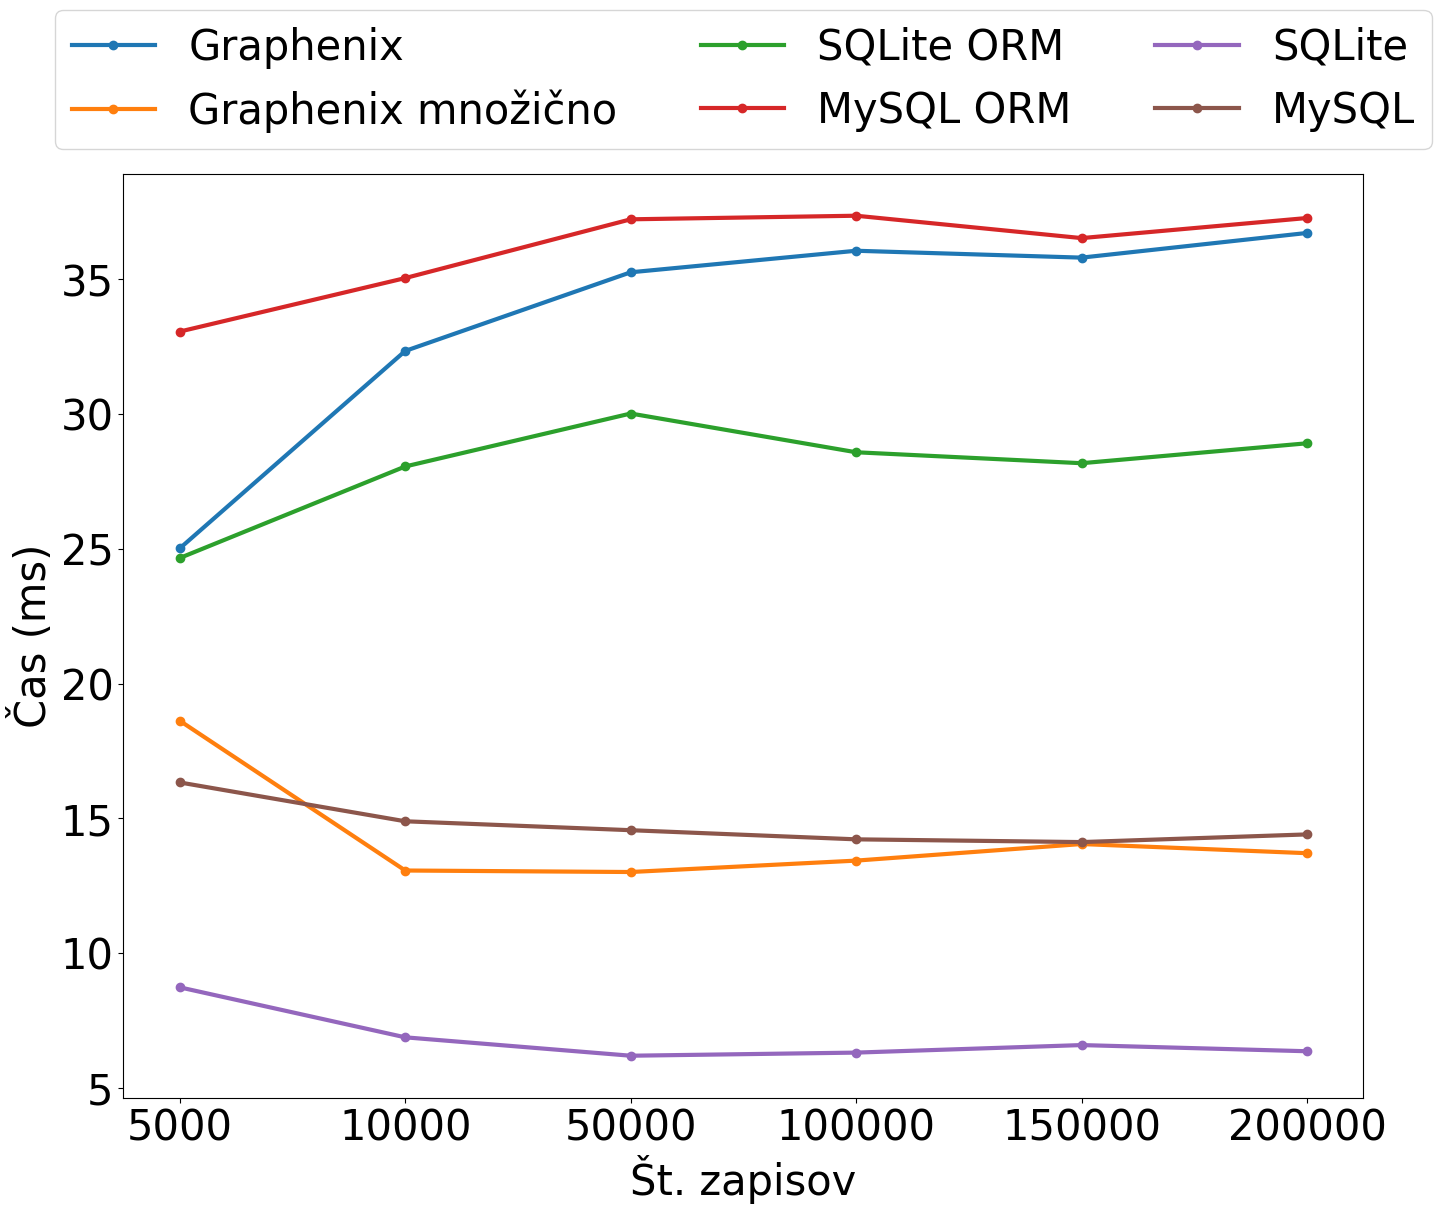
\includegraphics[width=0.6\textwidth, angle=0]{singleinsert.png}}
        \caption{Preprost primer relacijske podatkovne baze.}
        \label{vnospodatkov}
    \end{figure}
    
    \begin{figure}[H]
        \centerline{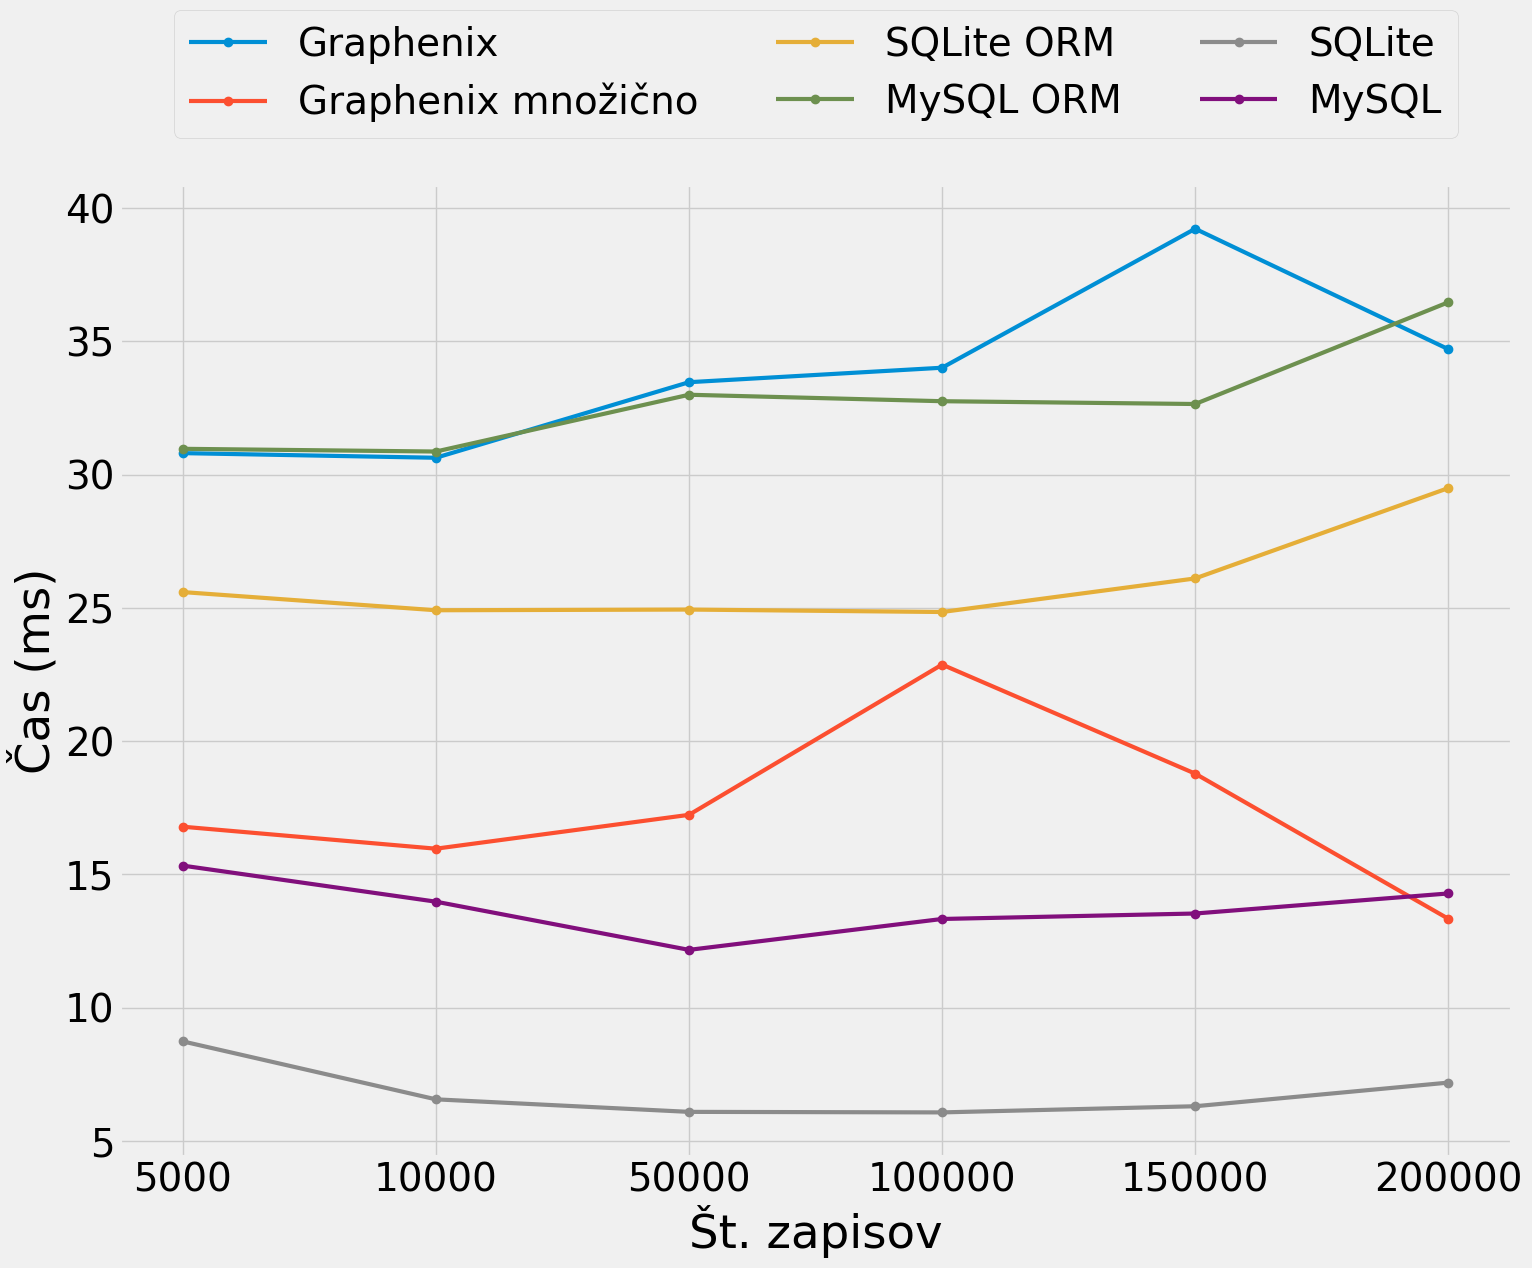
\includegraphics[width=0.6\textwidth, angle=0]{indexinsert.png}}
        \caption{Preprost primer relacijske podatkovne baze.}
        \label{vnospodatkov_index}
    \end{figure}

    \newpage
    \subsection{Velikosti podatkovnih sistemov na disku}
    \begin{figure}[H]
        \centerline{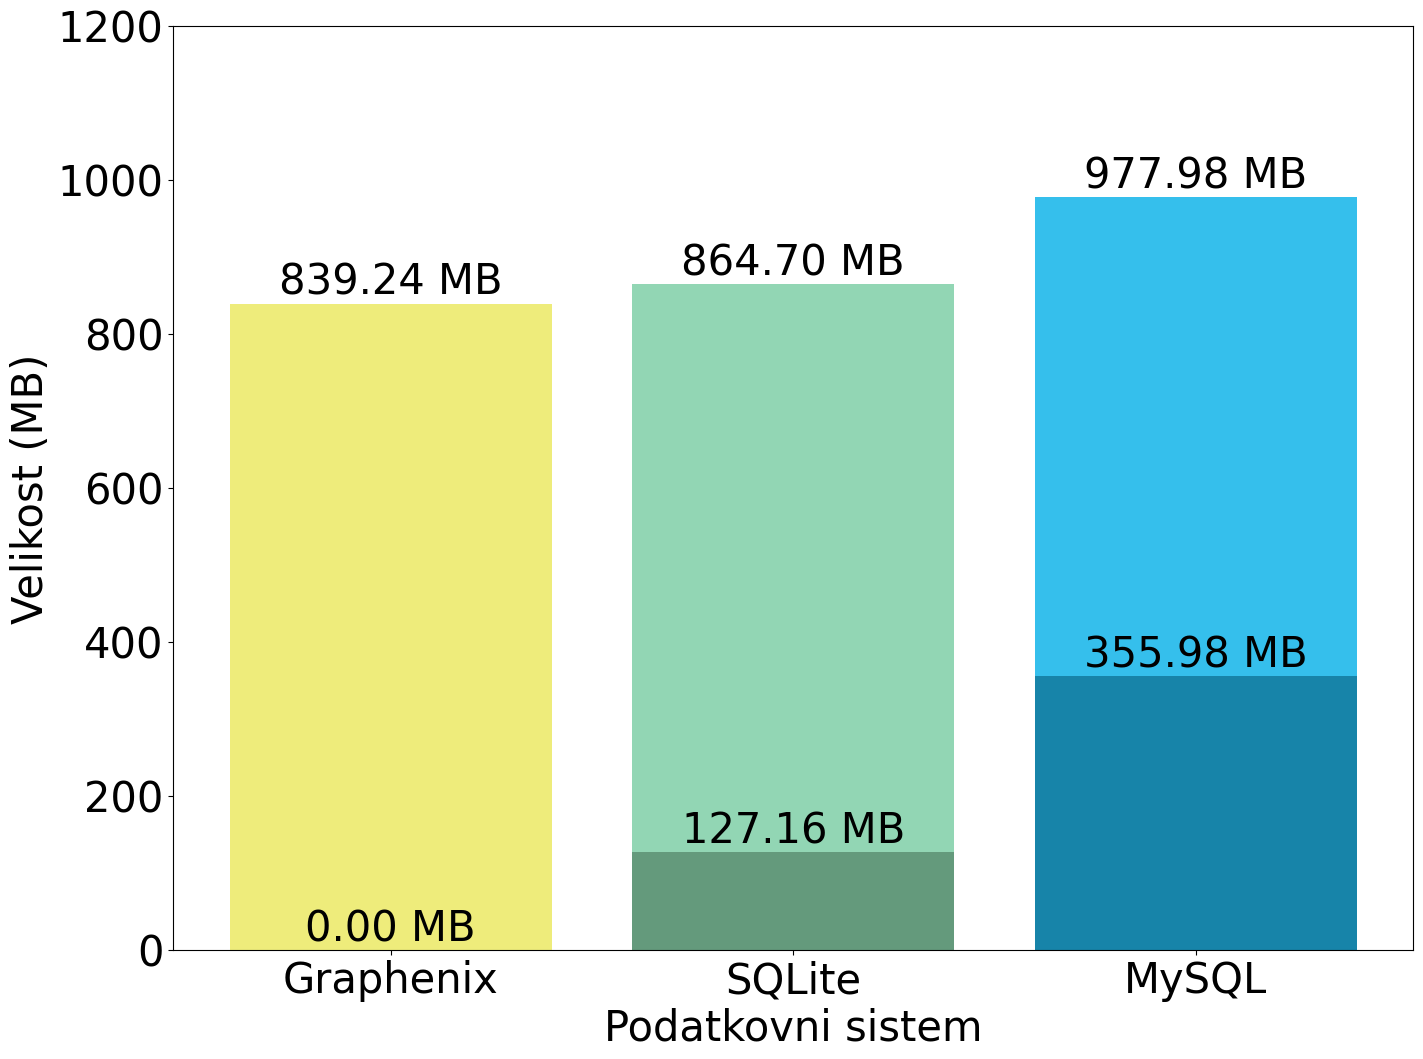
\includegraphics[width=0.6\textwidth, angle=0]{sizes.png}}
        \caption{Preprost primer relacijske podatkovne baze.}
        \label{vnospodatkov_index}
    \end{figure}

    \newpage
    \subsection{Primerjava poizvedb na eni entiteti}

    \begin{figure}[H]
        \centerline{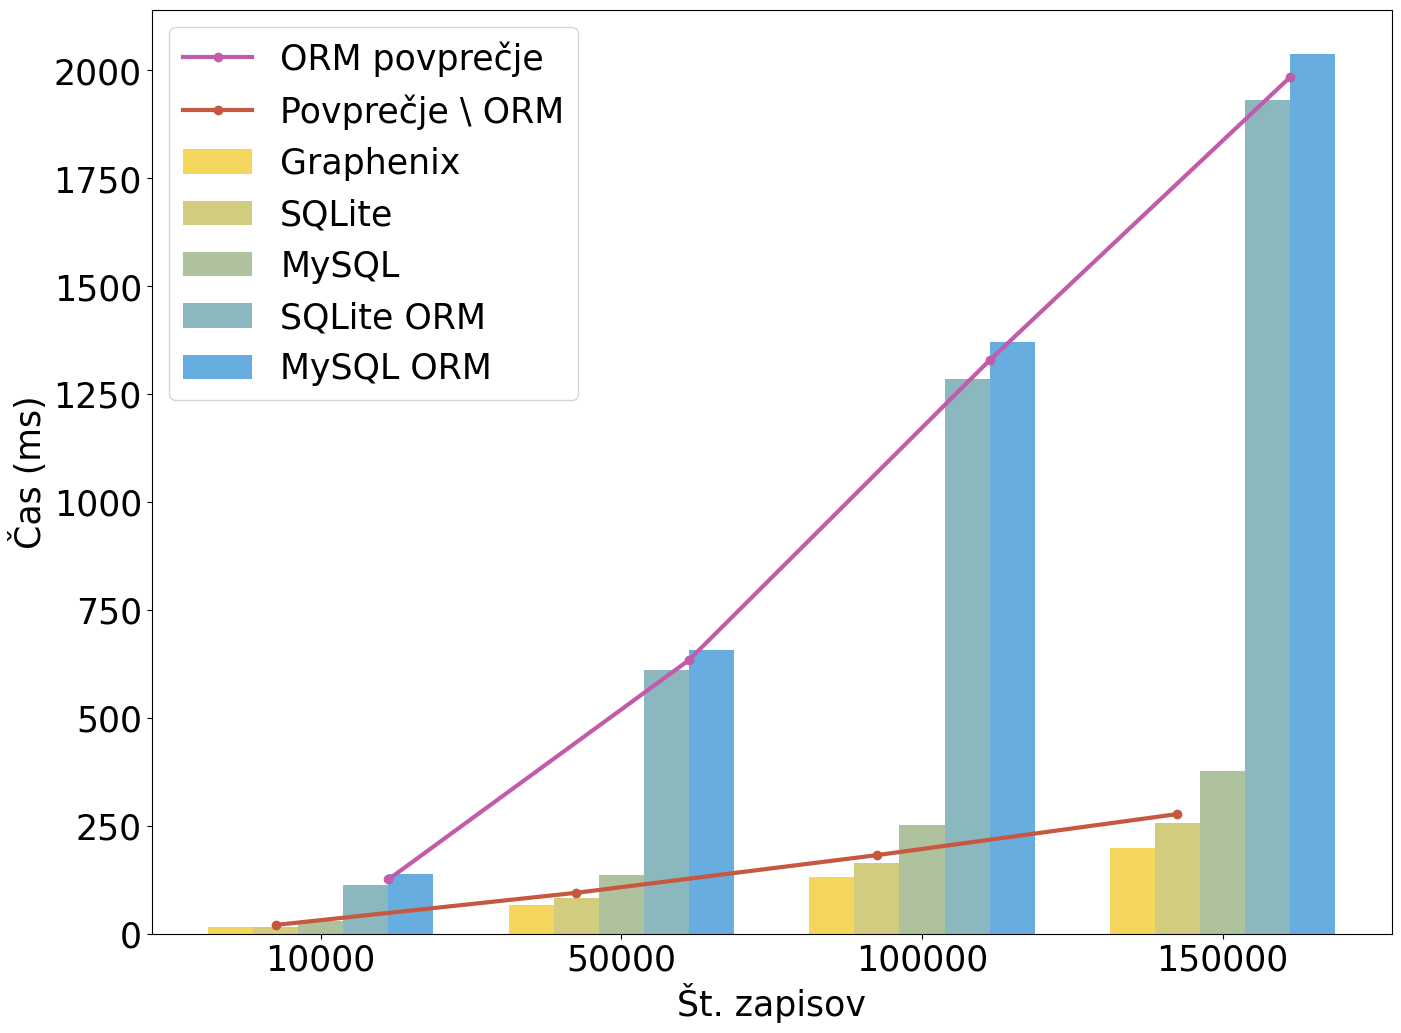
\includegraphics[width=0.6\textwidth, angle=0]{singleread.png}}
        \caption{Preprost primer relacijske podatkovne baze.}
        \label{vnospodatkov_index}
    \end{figure}

    \begin{figure}[H]
        \centerline{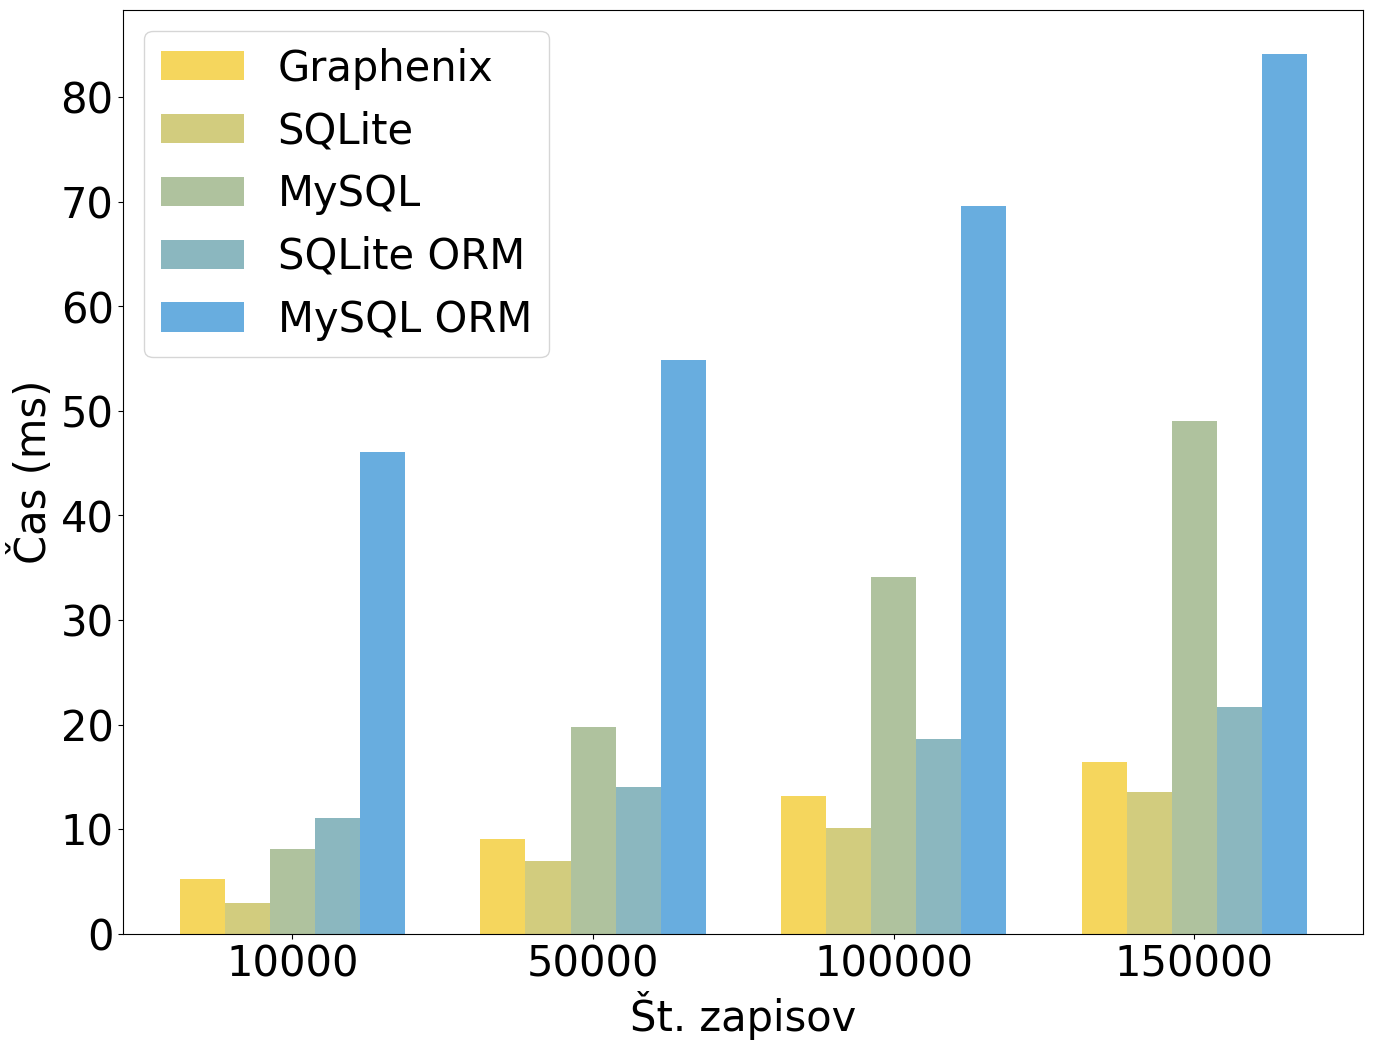
\includegraphics[width=0.6\textwidth, angle=0]{queryread.png}}
        \caption{Preprost primer relacijske podatkovne baze.}
        \label{vnospodatkov_index}
    \end{figure}

    \newpage
    \subsection{Primerjava poizvedb z uporabo relaciji}
    
    \newpage
    \subsection{Filtriranje podatkov s pomočjo indeksiranja}


    
\chapter{Scenariji oz. primeri uporabe}
\label{ch3}
    \section{Strežniško beleženje podatkov}

    Pogosta uporaba programskega jezika Python je na strani strežniških aplikaciji. Tukaj je beleženje vseh zapisov zelo pomembno torej vsakega zahtevka, časovne točke in odgovora na zahtevek. Z uporabo pripravljene knjižnice je prilagojeno beleženje podatkov lahko zelo preprosto.

    V prvi fazi si lahko pripravimo preprosto strežniško aplikacijo, ki ima vsega eno točko za pridobivanje podatkov in sicer ``get-range``, kjer lahko sami definiramo 3 argumente, to so ``start``, ``end`` in ``step``, kjer ima vsak od teh argumentov tudi privzete vrednosti.

    \subsection{Aplikacija, ki služi kot osnova za modul beleženja}
\begin{minted}{python}
app = Flask(__name__)
@app.route('/get-range')
def get_range(request):
    start = int(request.args.get('start', 0))
    end = int(request.args.get('end', 10))
    step = int(request.args.get('step', 1))
    return jsonify({'Range': list(range(start, end, step))})
app.run()
\end{minted}

    \noindent
    Zelo preprost pristop dodajanja beleženja je z uporabo vzorca dekoratorjev, ki omogočajo dodajanje funkcionalnosti na izbrane vhodne točke naše strežniške aplikacije. V zgornjem primeru že imamo primer dekoratorja in sicer $@app.route(...)$, ki funkcijo označi, kot vhodno točko za našo strežniško aplikacijo. Za naš primer bomo na vsako vhodno točko strežniške aplikacije dodali dekorator, kjer se za vsakim odgovorom zapiše HTTP pot, trenutni čas, parametri v zahtevku, odgovor in status le-tega. V prvi fazi rabimo najprej kreirati shemo za shranjevanje podatkov, ter potrebno entiteto, kjer bomo držali podatke o zahtevkih.

    \subsection{Kreiranje sheme za beleženje podatkov}
\begin{minted}{python}
class ReqInfo(Model):
    route = Field.String(size=255)
    timestamp = Field.DateTime().as_index()
    route_req = Field.String(size=1024)
    route_res = Field.String(size=1024)
    resp_code = Field.Int()

logging = Schema('logging', models=[ReqInfo])
if not logging.exists():
    logging.create()
\end{minted}

    \noindent
    V zgornjem segmentu pripravimo razred, ki predstavlja entiteto s posameznimi atributi, ki predstavljajo podatke, katere bomo tekom delovanja naše aplikacije beležili. V drugi fazi, pa moramo kreirati celotno shemo, kjer definiramo naziv celotne sheme in pa vse razrede oz. entitete, ki bodo uporabljene znotraj naše sheme.

    \newpage
    \subsection{Dekorator za dinamično dodajanje beleženja}

\begin{minted}{python}
def route_with_log(route):
    def decorator(f):
        @wraps(f)
        def wrapper(*args, **kwargs):
            try:
                response = f(request, *args, **kwargs)
            except Exception as err:
                response = None

            ReqInfo(
                route=route,
                timestamp=datetime.now(),
                route_req=json.dumps(dict(request.args)),
                route_res=response.get_data(as_text=True) if response else '',
                resp_code=response.status_code if response else 500
            ).make()

            return response
        
        app.add_url_rule(route, view_func=wrapper)
        return wrapper
    return decorator
\end{minted}

    \noindent
    Dekorator je v vzorec, kjer funkcija vrača drugo funkcijo in predstavlja nek ovoj funkcije. Tekom izvedbe ovite funkcije lahko argumente in različne segmente izvajanja prestrežemo in jih prilagodimo glede na naše zahteve. Pogosta uporaba vzorca, je tudi ko želimo na različne akcije dodati različne zahteve npr. strežniški vhodni točki želimo dodati preverjanje, če je uporabnik prijavljen z uporabo žetona in v primeru, ko uporabnik ni prijavljen v funkcijo vrinemo funkcionalnost, ki zavrne zahtevo uporabnika in vrne status 401 (ne prijavljen uporabnik). V primeru našega dekoratorja, pa lahko dekorator $@app.route(...)$ preprosto zamenjamo z $route\_with\_log(...)$ in funkcija bo ohranila tip vhodne točke, poleg tega pa dobi tudi funkcionalnost beleženja podatkov.

    \subsection{Branje zapisanih podatkov}

    V končni fazi je glavna prednost uporabe pripravljene knjižnice za beleženje podatkov struktura shranjenih podatkov. Namreč z uporabo relacijskega podatkovnega sistema dosežemo fiksno strukturo, ki je v primeru klasičnih datotek za beleženje nimamo. Omogočeno nam je tudi bistveno več načinov pridobivanja statistik na nivoju naše strežniške aplikacije, saj lahko podatke filtriramo in po potrebi dodamo še indeksiranje na stolpce, po katerih pogosteje iščemo in urejamo podatke npr. čas zahtevka (timestamp). Na nivoju administratorske aplikacije lahko nato prožimo različne poizvedbe nad $ReqInfo$ entiteto.

    \subsubsection{Izpis zadnjih treh zahtevkov}

\begin{minted}{python}
# izpis zadnjih treh zahtevkov
_, reqs = ReqInfo.order(ReqInfo.timestamp.desc()).limit(3).all()
\end{minted}

\begin{minted}{python}
ReqInfo(id=3, route=/get-range, timestamp=2023-07-16 03:02:15, 
    route_req={}, route_res={"Range":[0,1,2,3,4,5,6,7,8,9]},
    resp_code=200)
    
ReqInfo(id=2, route=/get-range, timestamp=2023-07-16 03:02:13, 
    route_req={"start": "3"}, route_res={"Range":[3,4,5,6,7,8,9]},
    resp_code=200)
    
ReqInfo(id=1, route=/get-range, timestamp=2023-07-16 03:02:05,
    route_req={"start": "15", "end": "10", "step": "-3"},
    route_res={"Range":[15,12]}, resp_code=200)
\end{minted}

    \subsubsection{Statističen pregled zahtevkov}

    Podatke lahko v vgrajenem podatkovnem sistemu tudi grupiramo, in sicer z uporabo $.agg(...)$ metode v poizvedbi, lahko definiramo polje po katerem grupiramo podatke, kot tudi agregacije, ki jih želimo izvesti.
    
\begin{minted}{python}
route_stats = ReqInfo\
    .agg(by=ReqInfo.route, count=AGG.count())
\end{minted}

    \subsubsection{Izpis napak v zadnjem dnevu}

    Za nabor napak v zadnjem dnevu, lahko preprosto izvedemo poizvedbo, kjer zahtevamo, da je status odgovora $>= 400$, kar pri HTTP zahtevkih predstavlja razpon napak. Poleg tega, pa dodamo še zahtevo, da mora biti datum napake večji, kot včerajšnji datum ob enaki uri. Za konec zapise uredimo po datumu napake.
    
\begin{minted}{python}
count, api_errors = ReqInfo\
    .filter(
        ReqInfo.resp_code >= 400,
        ReqInfo.timestamp > datetime.now() - timedelta(days=1)
    )\
    .order(ReqInfo.timestamp.desc())\
    .all()
\end{minted}

    \subsubsection{Izvoz vseh podatkov v .csv datoteko}

    Podatkovni sistem omogoča tudi izvoz v csv datoteko, ki za nekatere uporabnike lahko pomeni lažjo obdelavo podatkov, poleg tega, pa lahko predstavlja tudi varnostno kopijo podatkovne baze v ločeni datoteki.

    Za omenjeno nalogo potrebujemo najprej izvesti nabor vseh podatkov, nato pa s pomočjo privzetega pretvornika podatke izvozi v datoteko s pomočjo metode "dump2csv", ki prejme dva parametra – podatke in naziv izvozne datoteke.
    
\begin{minted}{python}
_, all_reqs = ReqInfo.all()
ViewSearilizer.default().dump2csv(all_reqs, 'export.csv')
\end{minted}

    \section{Manjši strežniški API}

    Strežniške aplikacije, ki zahtevajo fleksibilno in hitro delo s podatkovnim sistemom postajajo vse bolj pogoste. Python predstavlja enega izmed najpogosteje uporabljenih programskih jezikov na omenjenem področju. Obstaja tudi že ogromno pripravljenih knjižnic za izdelavo API aplikaciji, kot tudi za sam podatkovni sistem, ki se uporablja znotraj aplikacije.

    Tekom poglavja je predstavljena izdelava strežniške aplikacije, kjer uporabljamo Flask \cite{FLASK_GITHUB} ogrodje. Sama aplikacija, pa je namenjena delu z sistemu prefesorjev in laboratorijev.
    
    \subsection{Podatkovna shema za aplikacijo}

    V shemi imamo vsega dve tabeli, ki bosta držali podatke o profesorjih in laboratorijih.
\begin{minted}{python}
class Teacher(Model):
    full_name = Field.String(size=256)
    email = Field.String(size=128)
    laboratory = Field.Link()

class Laboratory(Model):
    name = Field.String(size=64)
    room_number = Field.Int()
    teachers = Field.VirtualLink('laboratory')
\end{minted}

    \newpage
    \subsection{Pretvornik za serializacijo podatkov nad shemo}

\begin{minted}{python}
class TeacherSearilizer(ViewSearilizer):
    fields = ('id', 'full_name', 'email')

class LaboratorySearilizer(ViewSearilizer):
    fields = '*'
    teachers = TeacherSearilizer
        
class BasicLaboratorySearilizer(ViewSearilizer):
    fields = ('id', 'name', 'room_number')

class DetailTeacherSearilizer(ViewSearilizer):
    fields = '*'
    laboratory = BasicLaboratorySearilizer
\end{minted}

    \subsection{Kreiranje novega zapisa}
    \subsection{Nabor podatkov profesorjev po laboratorijih}
    \subsection{Nabor podatkov z dinamičnim filtriranjem}

\chapter{Sklepne ugotovitve}
    \colorbox{BurntOrange}{Splošne ugotovitve tekom izdelave vgrajenega podatkovnega sistema}
    \newline
    \colorbox{BurntOrange}{in strnjene ugotovitve glede na analizo}

%\cleardoublepage
% \addcontentsline{toc}{chapter}{Literatura}

% če imaš težave poravnati desni rob bibliografije, potem odkomentiraj spodnjo vrstico
\raggedright

% v zadnji verziji diplomskega dela običajno združiš vse tri vrste referenc v en sam seznam in
% izpustiš delne sezname
\printbibliography[heading=bibintoc,title={Literatura}]

\end{document}